\documentclass[aspectratio=169]{beamer}
\usepackage[utf8]{inputenc}
\usetheme{Warsaw}
\usecolortheme{default}
\setbeamersize{text margin left=0pt,text margin right=0pt} 
\setbeamertemplate{navigation symbols}{}%remove navigation symbols

\usepackage{graphicx}
%\usepackage[caption=false]{subfig}

\usepackage[font={small}]{caption, subfig}
%\renewcommand{\figurename}{Figure}
%\renewcommand{\tablename}{Table}
\setlength{\abovecaptionskip}{-0.5ex}
\setlength{\belowcaptionskip}{-1ex}
\setlength{\floatsep}{0pt}
\setlength{\textfloatsep}{0pt}


\title[Data Governance for $\Phi$ BSA]{Data Governance for \texorpdfstring{$\Phi$}{Phi} Beam Spin Asymmetry}
\subtitle{Weekly Update}
\author{Paul Simmerling}
\institute[UConn]{University of Connecticut}
\date{November 26, 2020}

\begin{document}
\frame{\titlepage}


\begin{frame}{Exclusivity Cuts \hfill Skim4 FD}
\vspace*{-0.6cm}
    \begin{columns}
    \column{0.5\textwidth}
    \begin{figure}
        \centering
        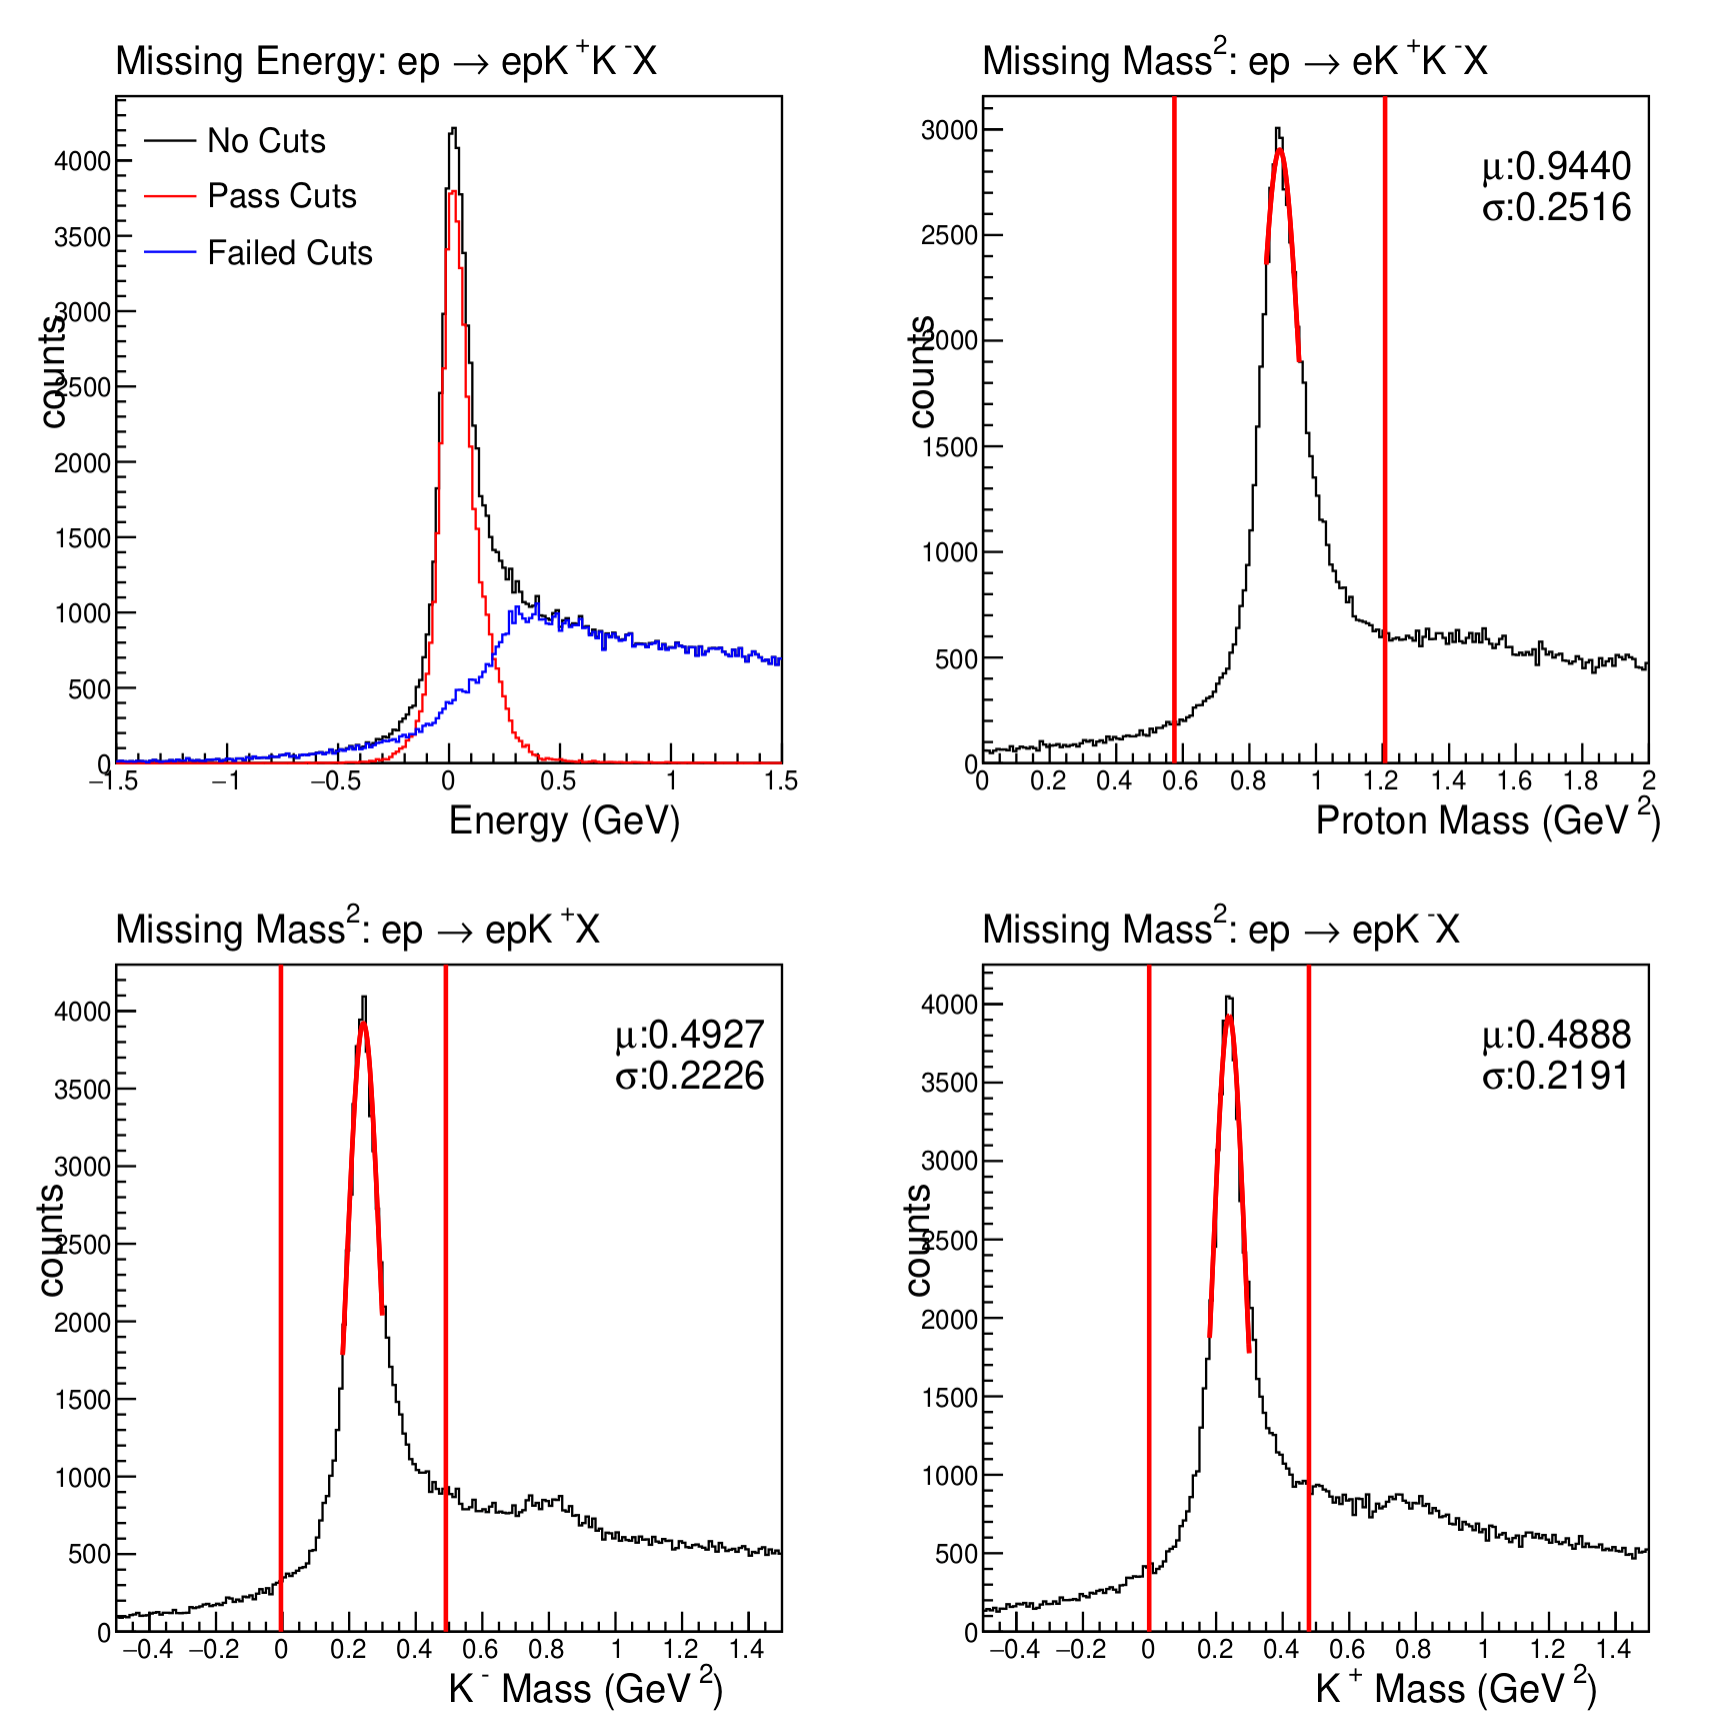
\includegraphics[width=0.94\textwidth]{brandon_figs/32a.png}
        \caption{Brandon 3.32a}
    \end{figure}
    \column{0.5\textwidth}
    \begin{figure}
        \centering
        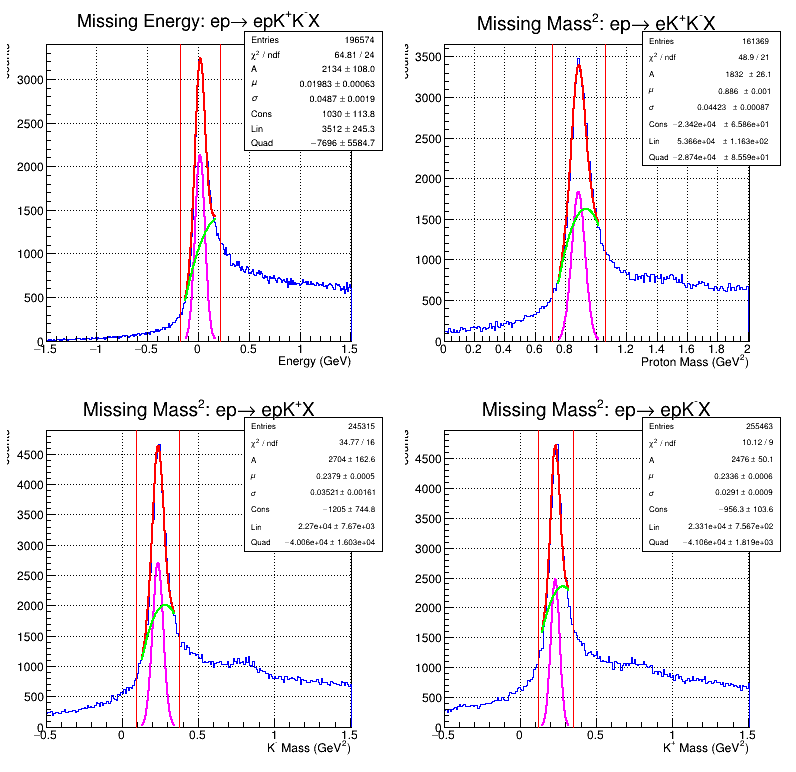
\includegraphics[width=0.97\textwidth]{pdfs/32a.png}
        \caption{My Reproduction}
    \end{figure}
    \end{columns}
\end{frame}

\begin{frame}{Exclusivity Cuts \hfill Skim4 FD}
\vspace*{-0.6cm}
    \begin{columns}
    \column{0.5\textwidth}
    \begin{figure}
        \centering
        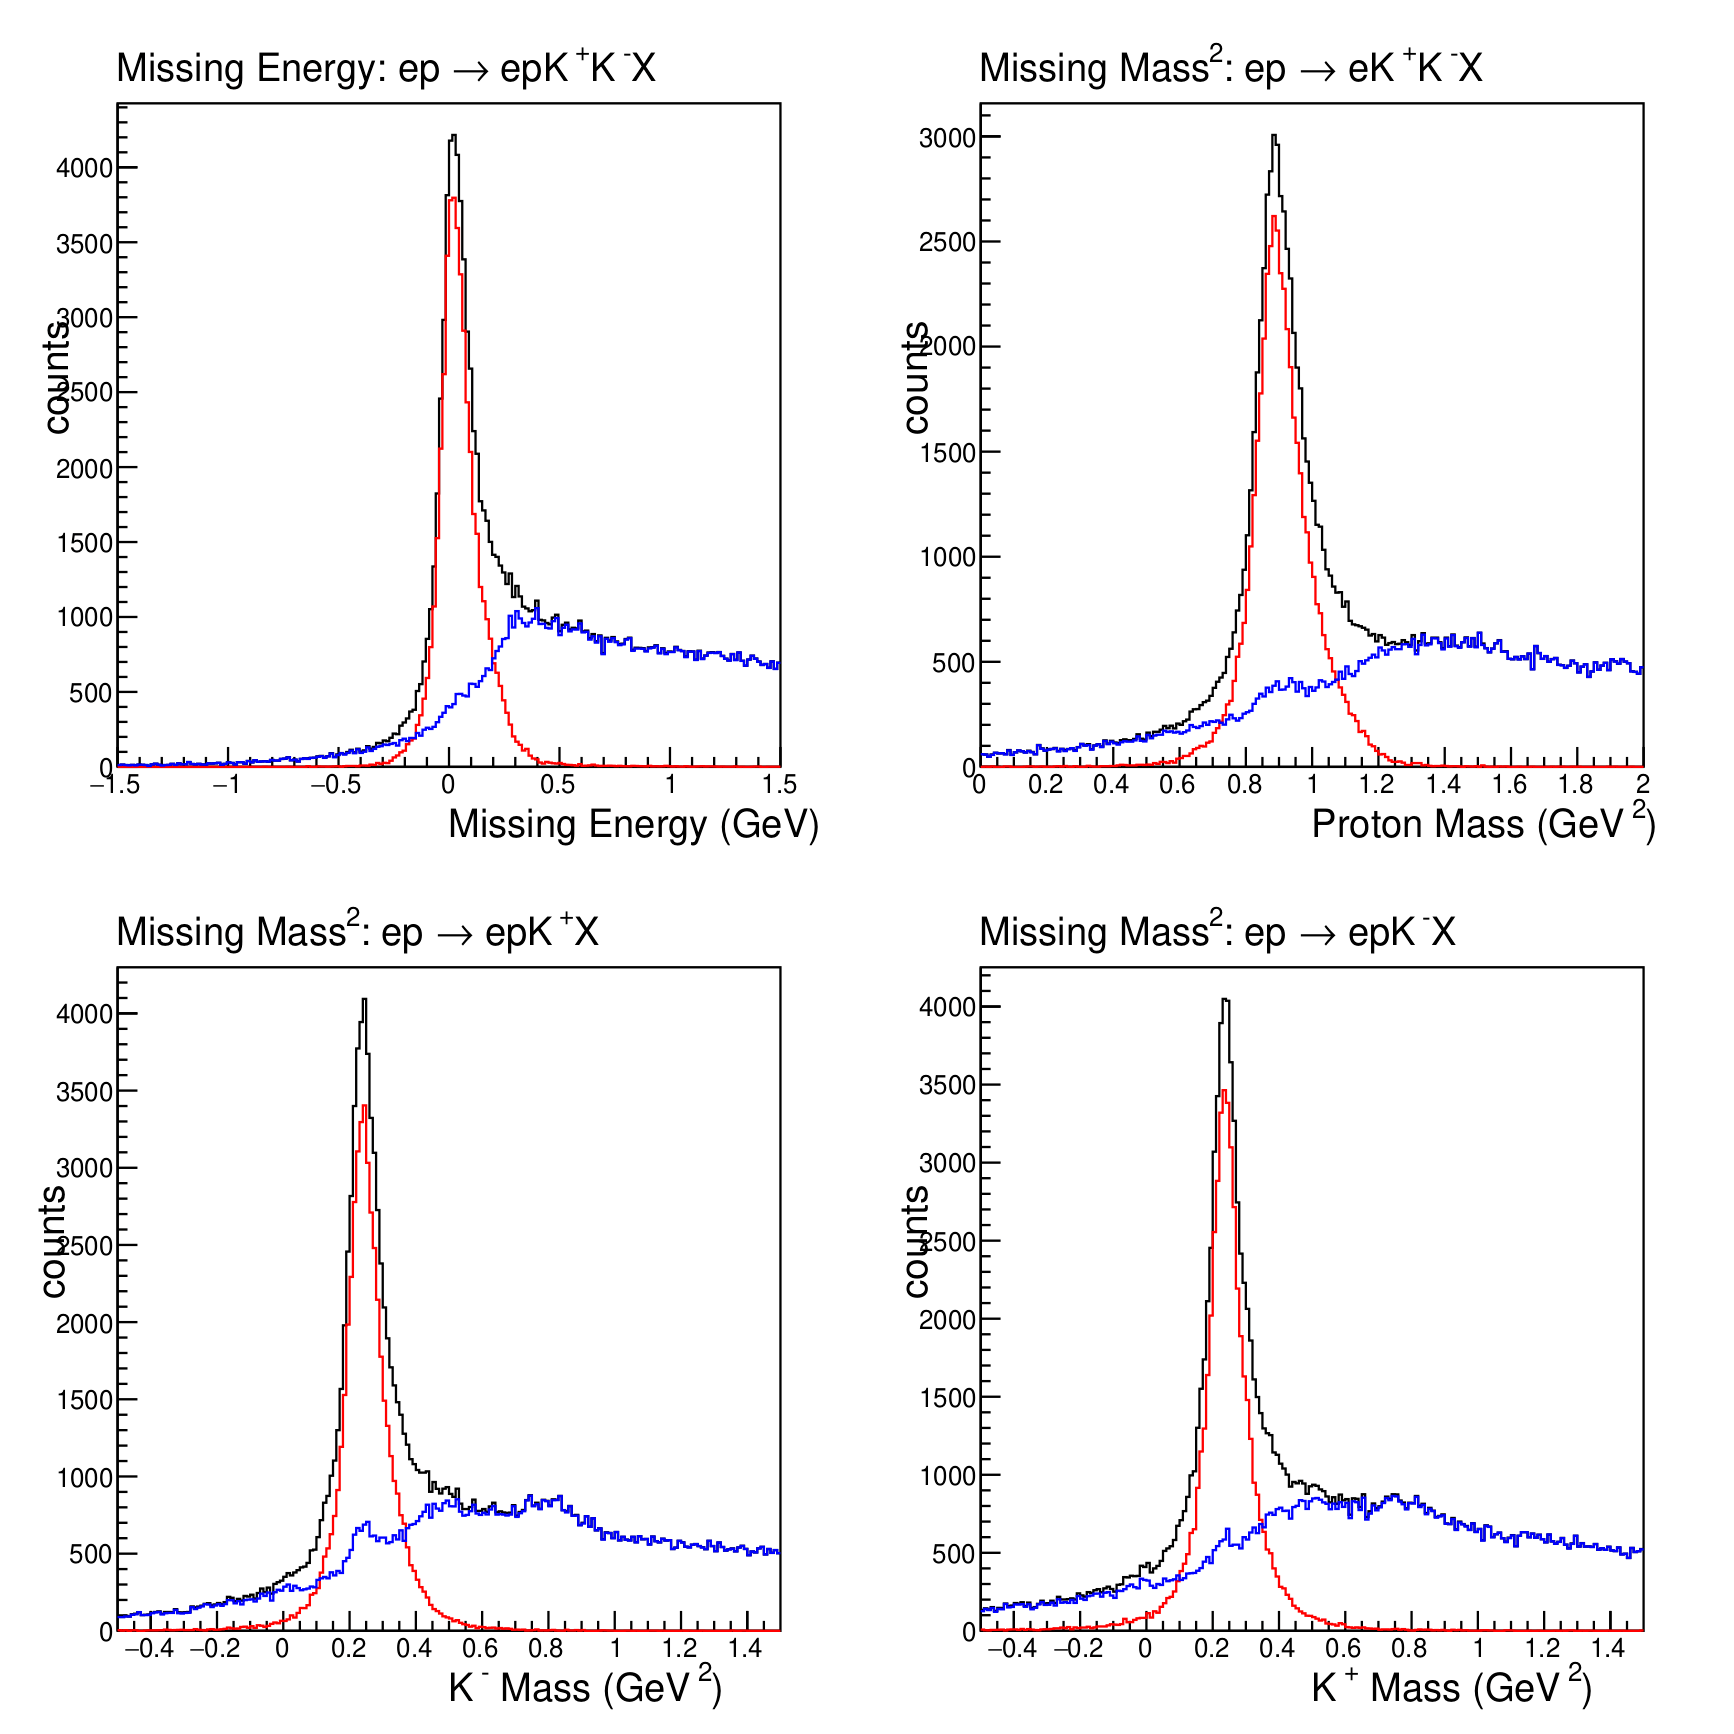
\includegraphics[width=0.94\textwidth]{brandon_figs/32b.png}
        \caption{Brandon 3.32b}
    \end{figure}
    \column{0.5\textwidth}
    \begin{figure}
        \centering
        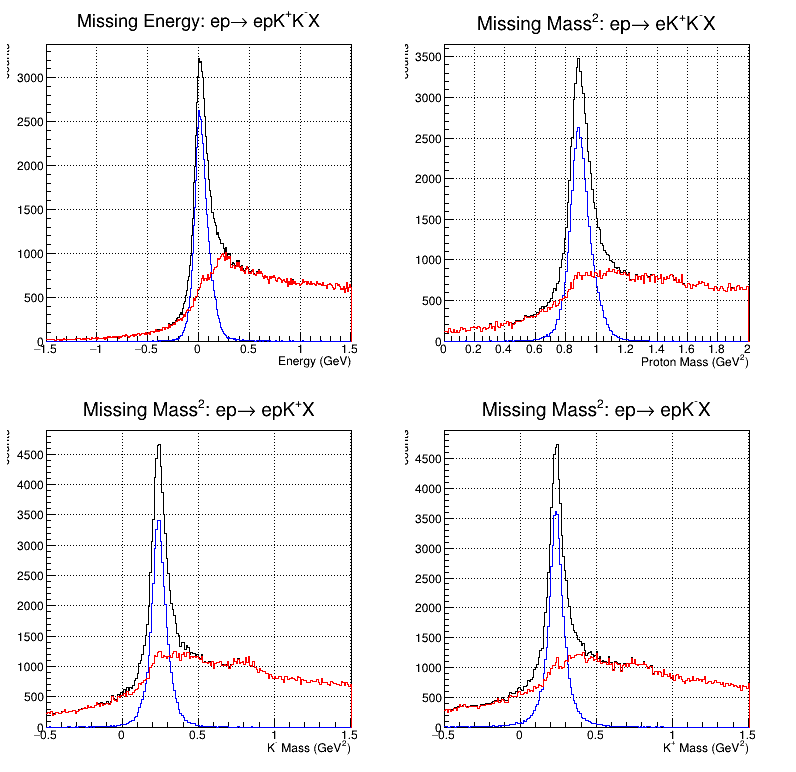
\includegraphics[width=0.97\textwidth]{pdfs/32b.png}
        \caption{My Reproduction}
    \end{figure}
    \end{columns}
\end{frame}

\begin{frame}{Vertex Difference Cut on Charged Kaons \hfill Skim4 FD}
\vspace*{-0.6cm}
    \begin{columns}
    \column{0.5\textwidth}
    \begin{figure}
        \centering
        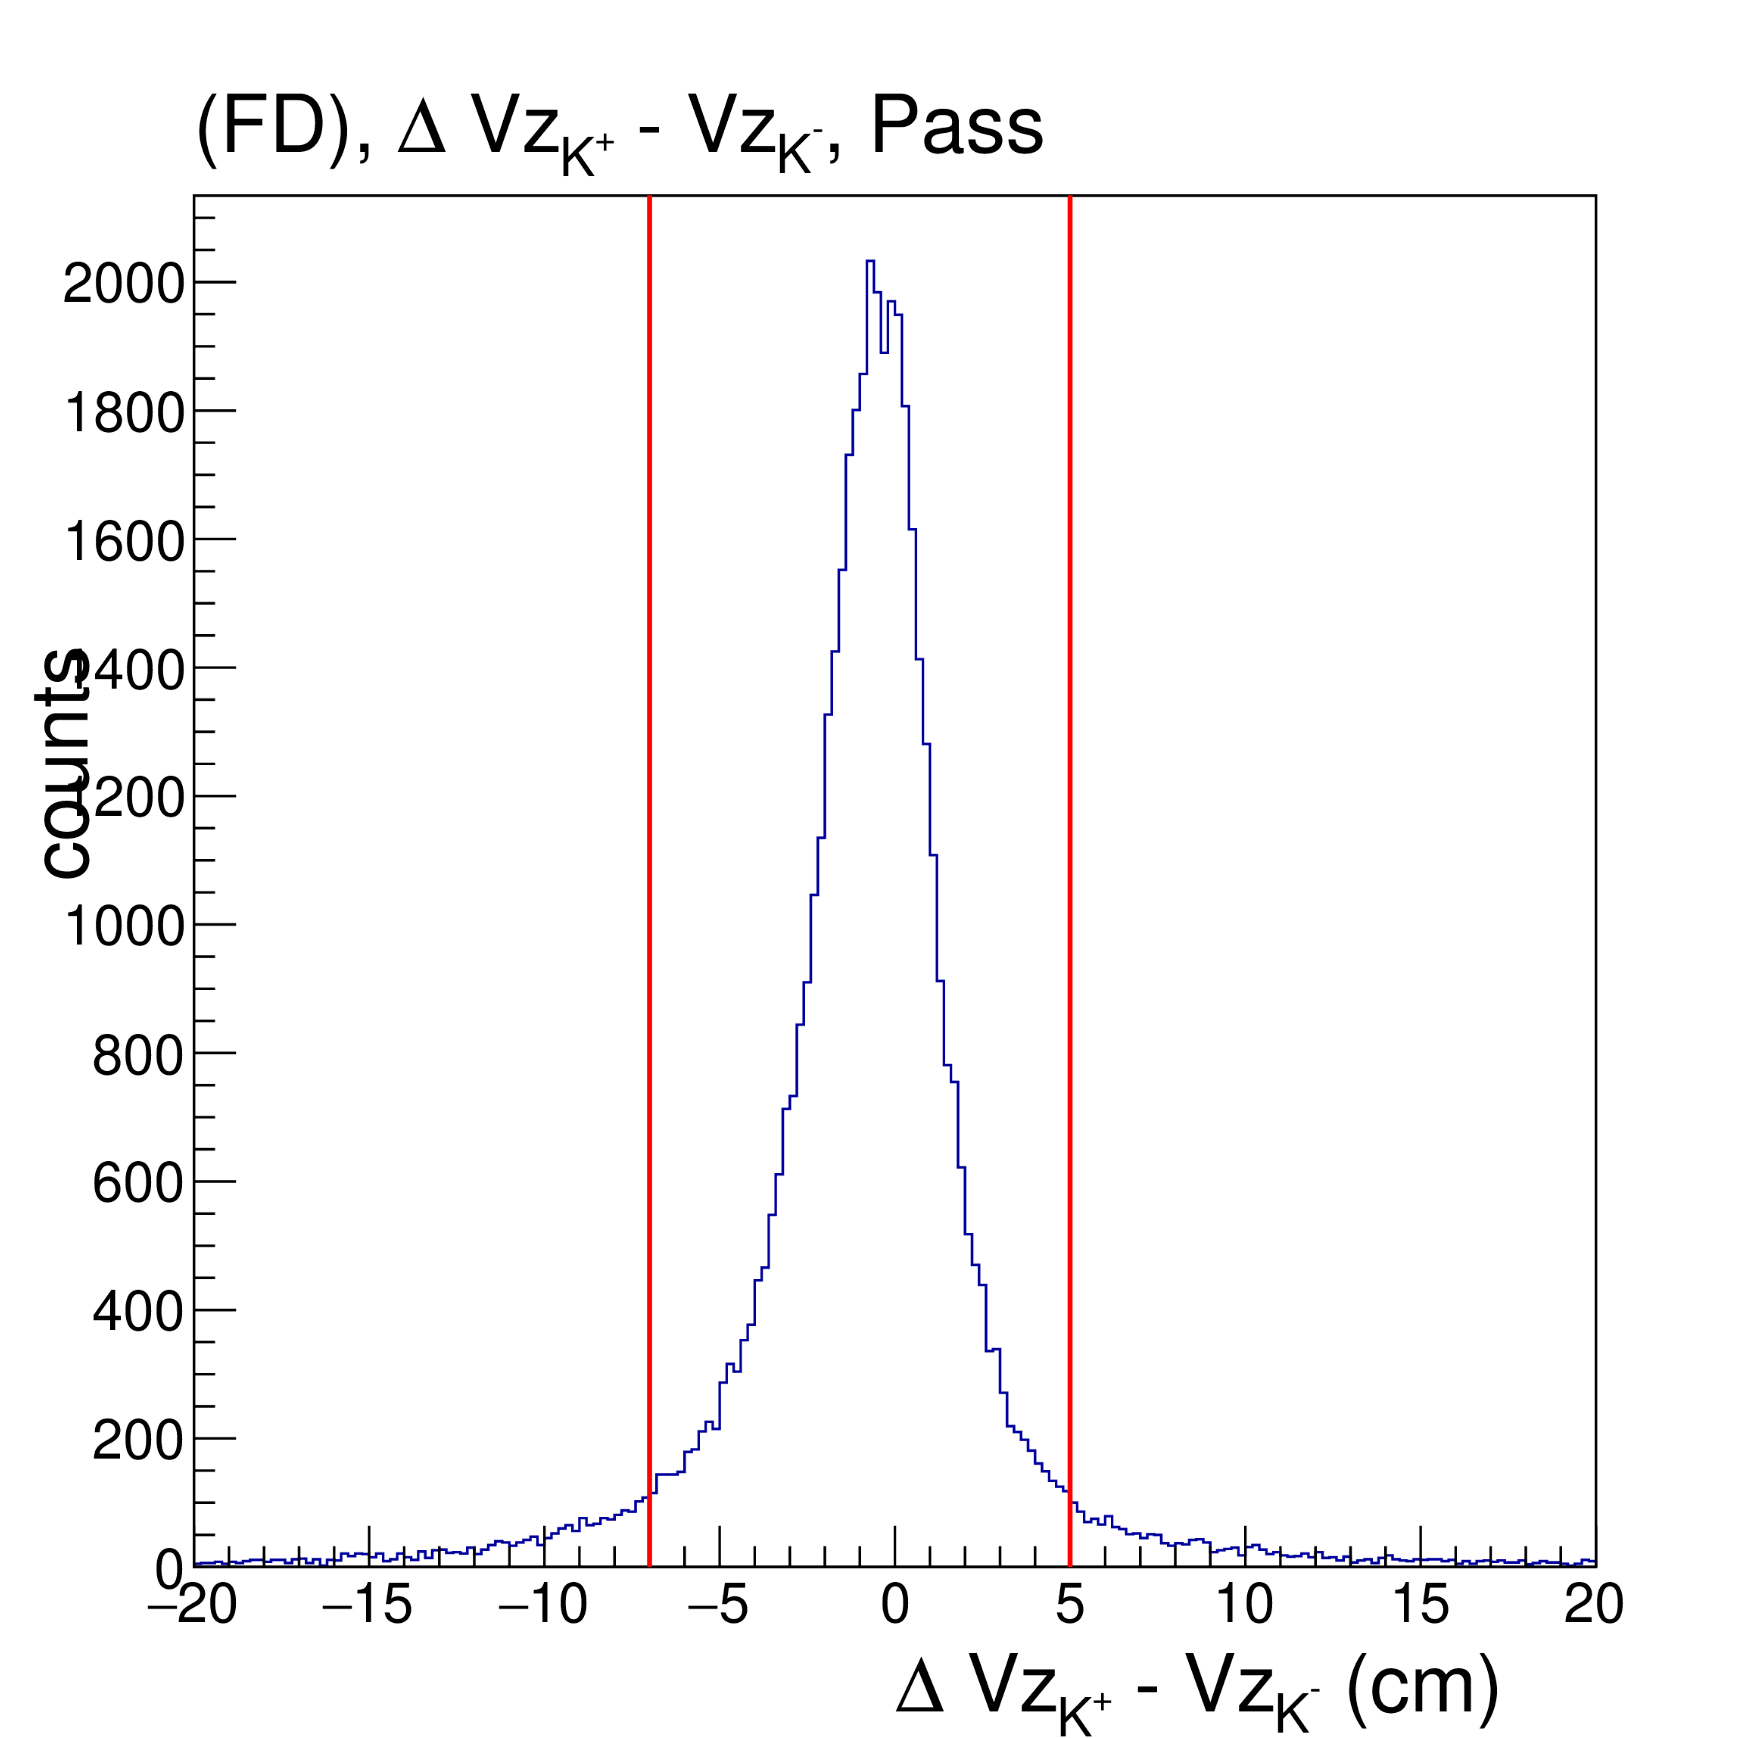
\includegraphics[width=0.94\textwidth]{brandon_figs/34a.png}
        \caption{Brandon 3.34a}
    \end{figure}
    \column{0.5\textwidth}
    \begin{figure}
        \centering
        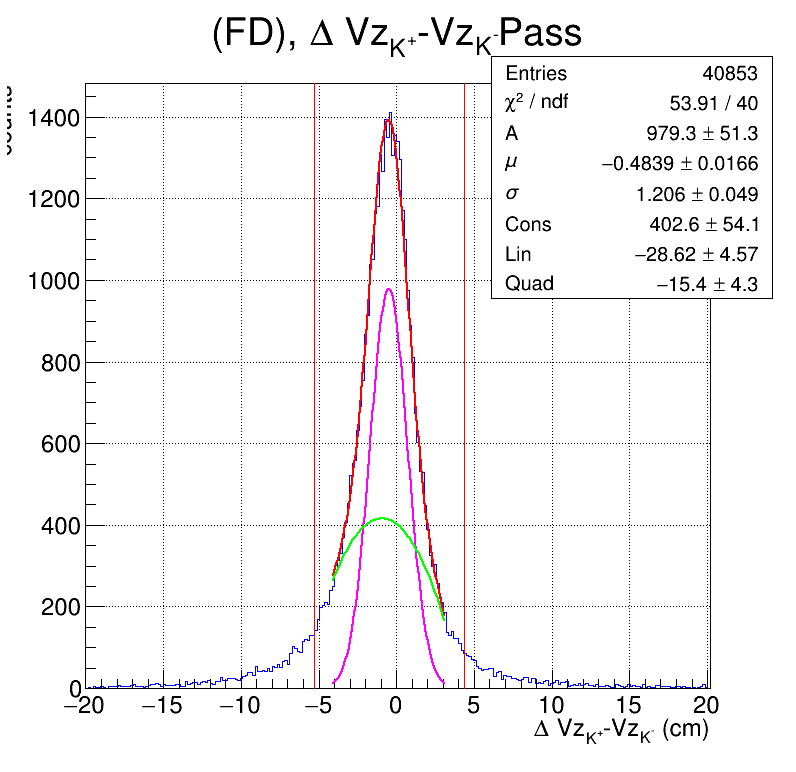
\includegraphics[width=0.97\textwidth]{pdfs/34a.png}
        \caption{My Reproduction}
    \end{figure}
    \end{columns}
\end{frame}

\begin{frame}{Vertex Difference Cut on Charged Kaons \hfill Skim4 FD}
\vspace*{-0.6cm}
    \begin{columns}
    \column{0.5\textwidth}
    \begin{figure}
        \centering
        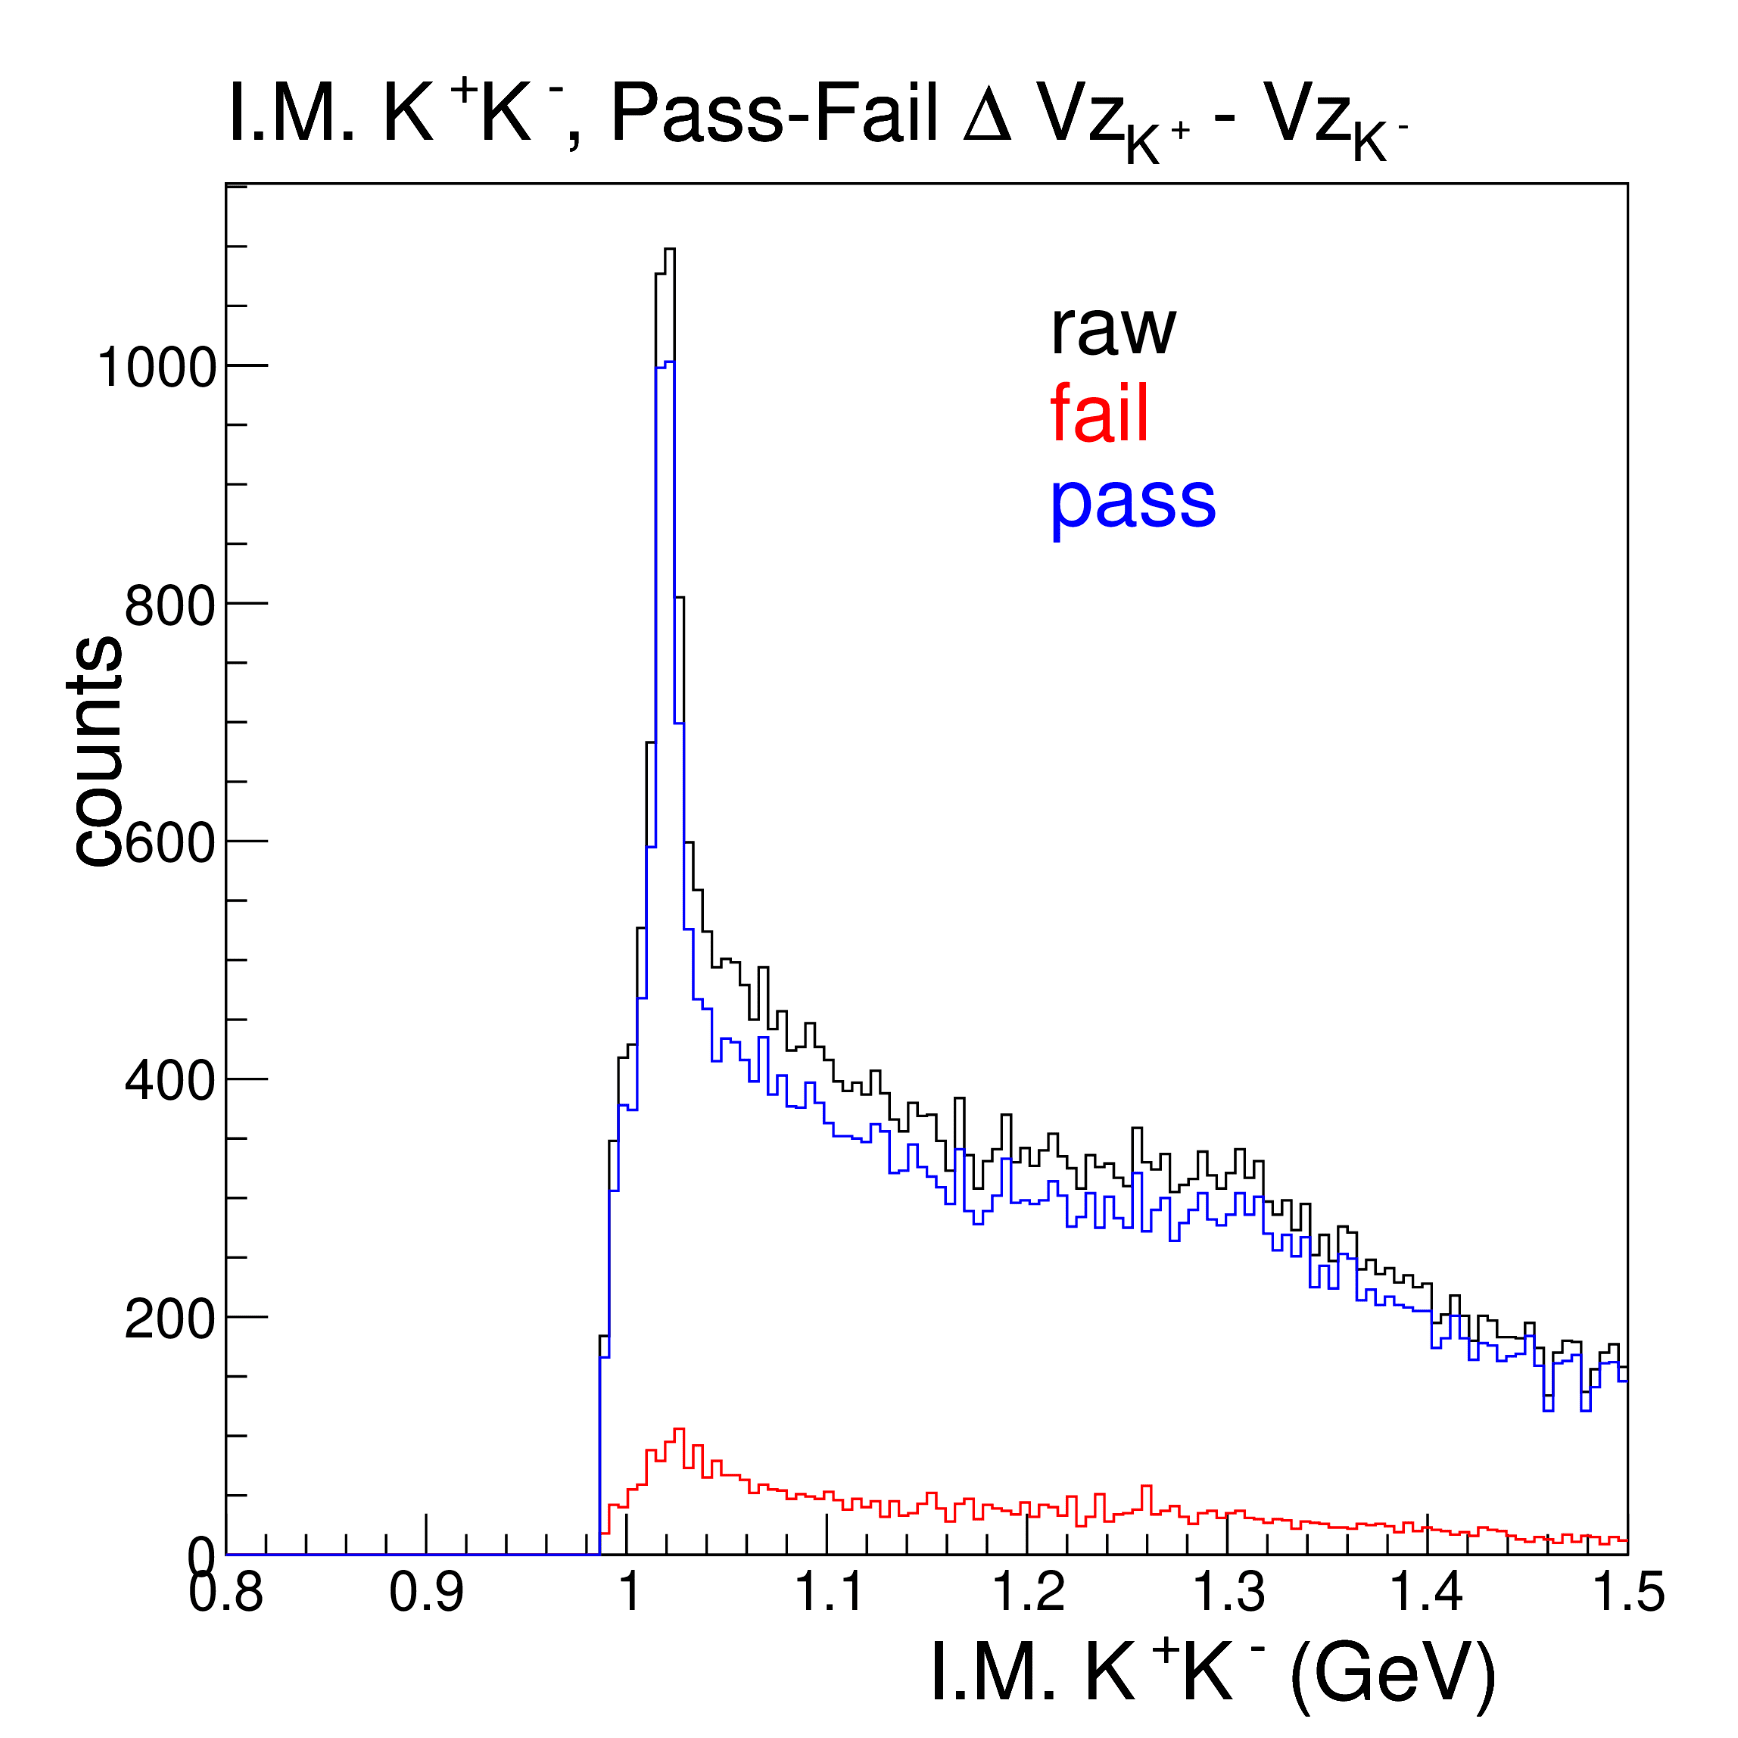
\includegraphics[width=0.94\textwidth]{brandon_figs/34b.png}
        \caption{Brandon 3.34b}
    \end{figure}
    \column{0.5\textwidth}
    \begin{figure}
        \centering
        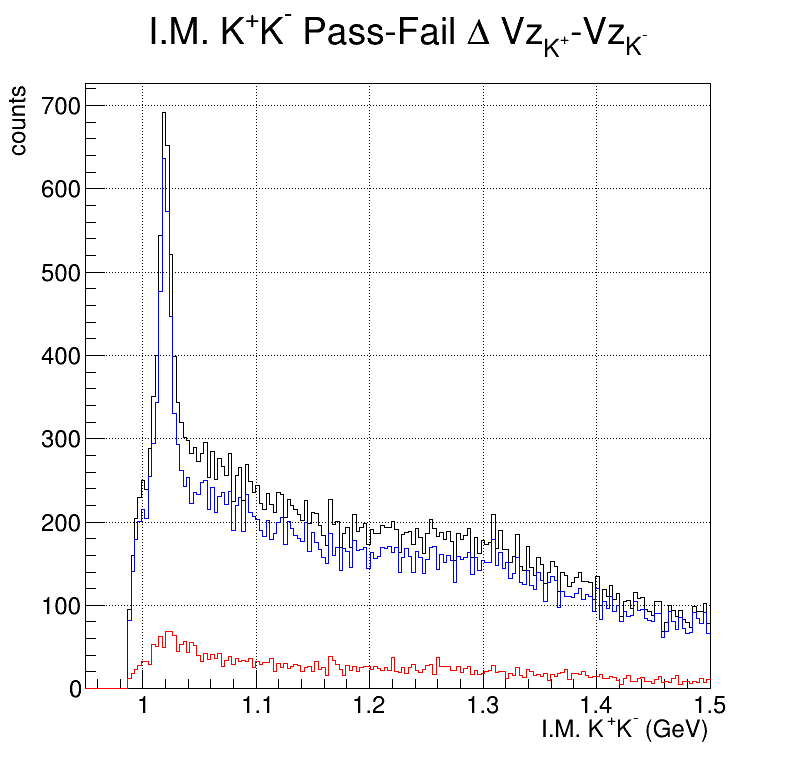
\includegraphics[width=0.97\textwidth]{pdfs/34b.png}
        \caption{My Reproduction}
    \end{figure}
    \end{columns}
\end{frame}

\begin{frame}{Coplanarity Cuts \hfill Skim4 FD}
\vspace*{-0.6cm}
    \begin{columns}
    \column{0.5\textwidth}
    \begin{figure}
        \centering
        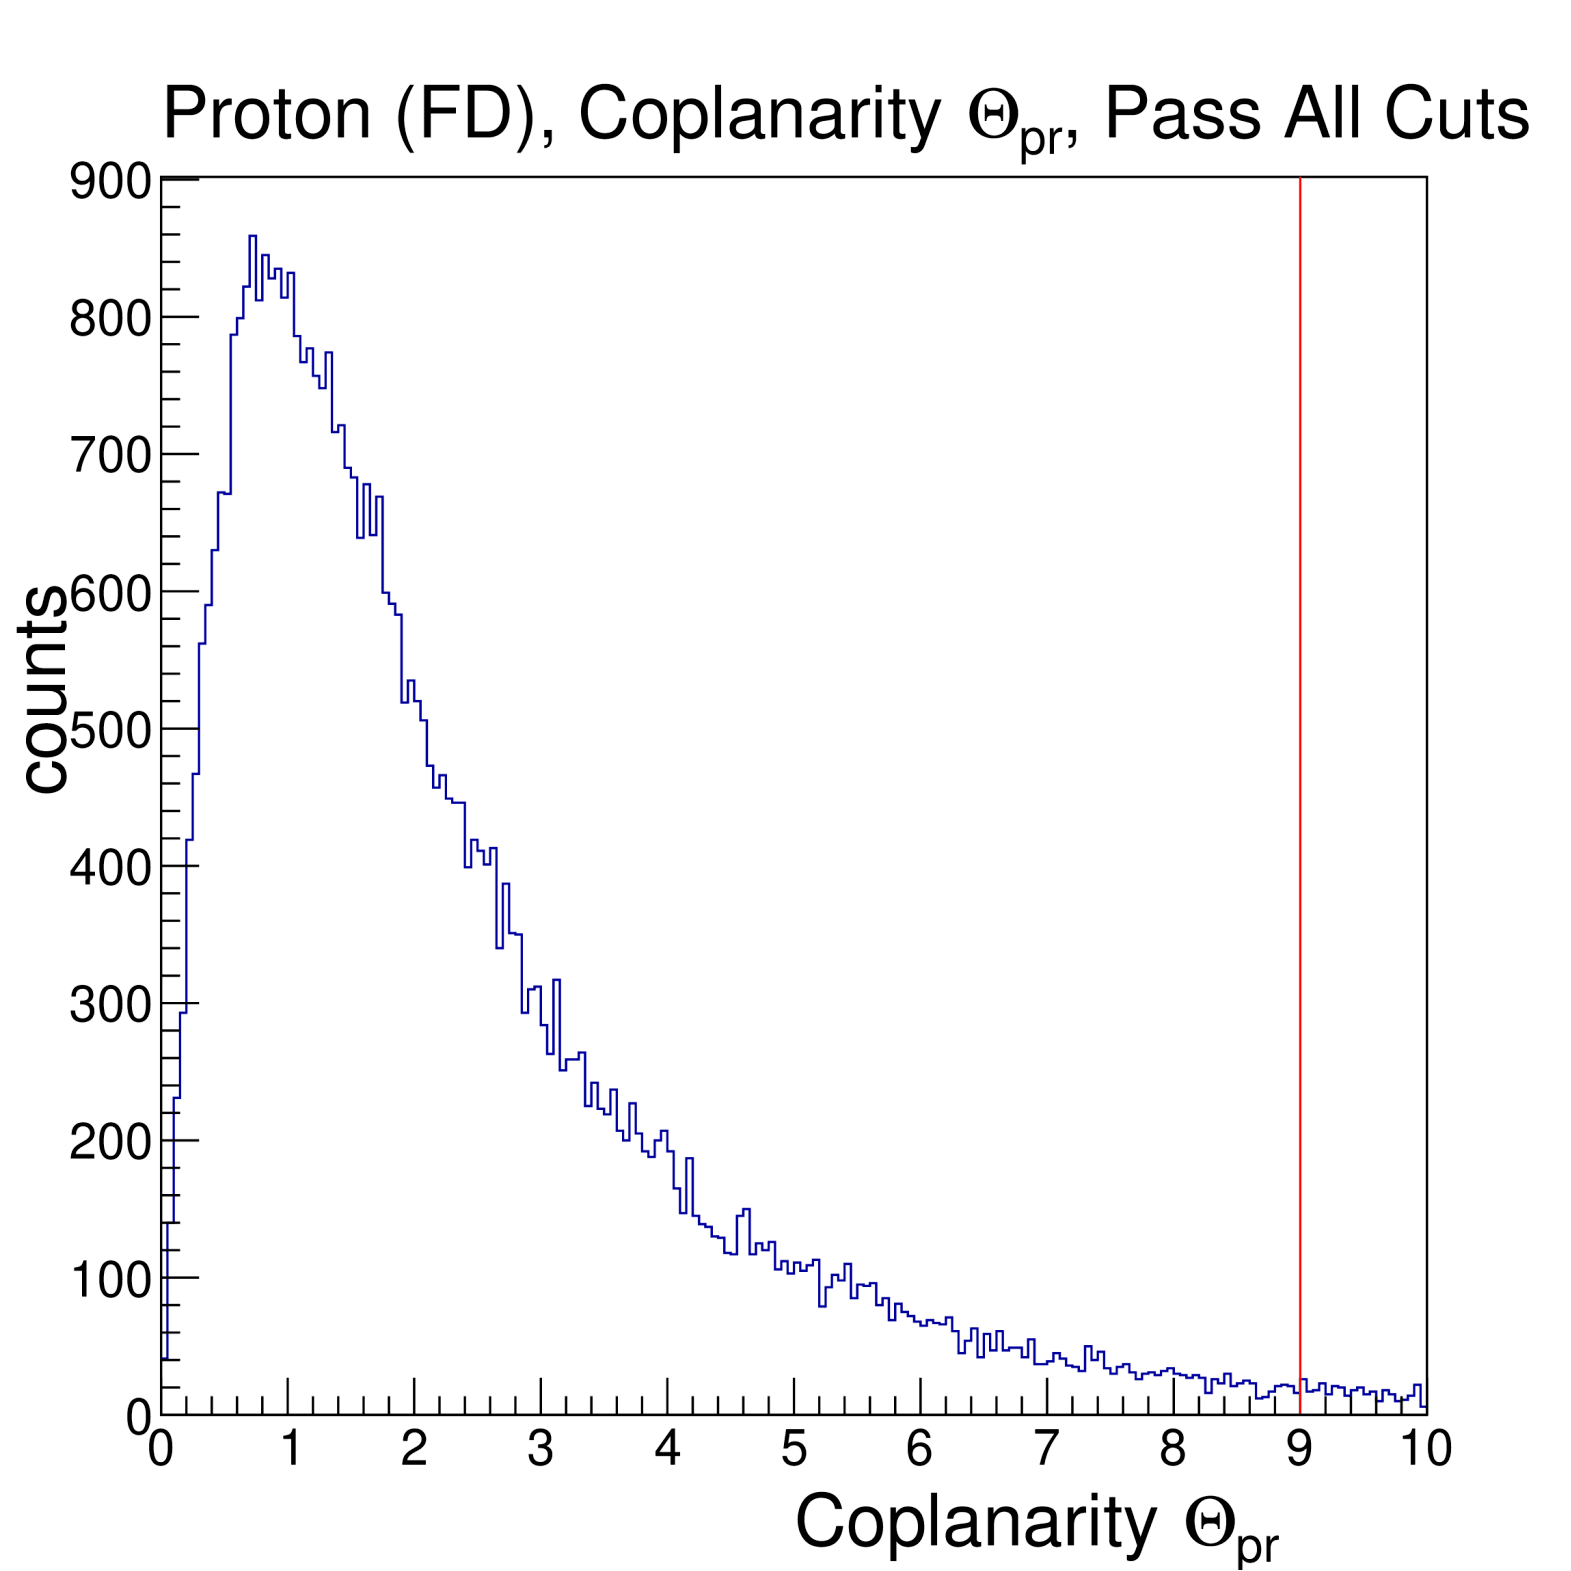
\includegraphics[width=0.94\textwidth]{brandon_figs/35a.png}
        \caption{Brandon 3.35a}
    \end{figure}
    \column{0.5\textwidth}
    \begin{figure}
        \centering
        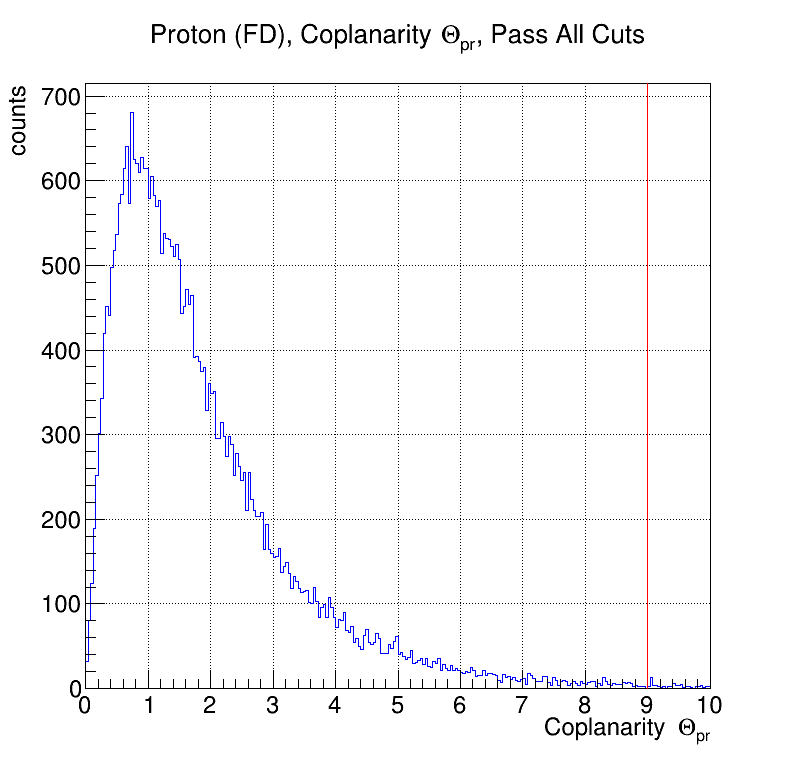
\includegraphics[width=0.97\textwidth]{pdfs/35a.png}
        \caption{My Reproduction}
    \end{figure}
    \end{columns}
\end{frame}

\begin{frame}{Coplanarity Cuts \hfill Skim4 FD}
\vspace*{-0.6cm}
    \begin{columns}
    \column{0.5\textwidth}
    \begin{figure}
        \centering
        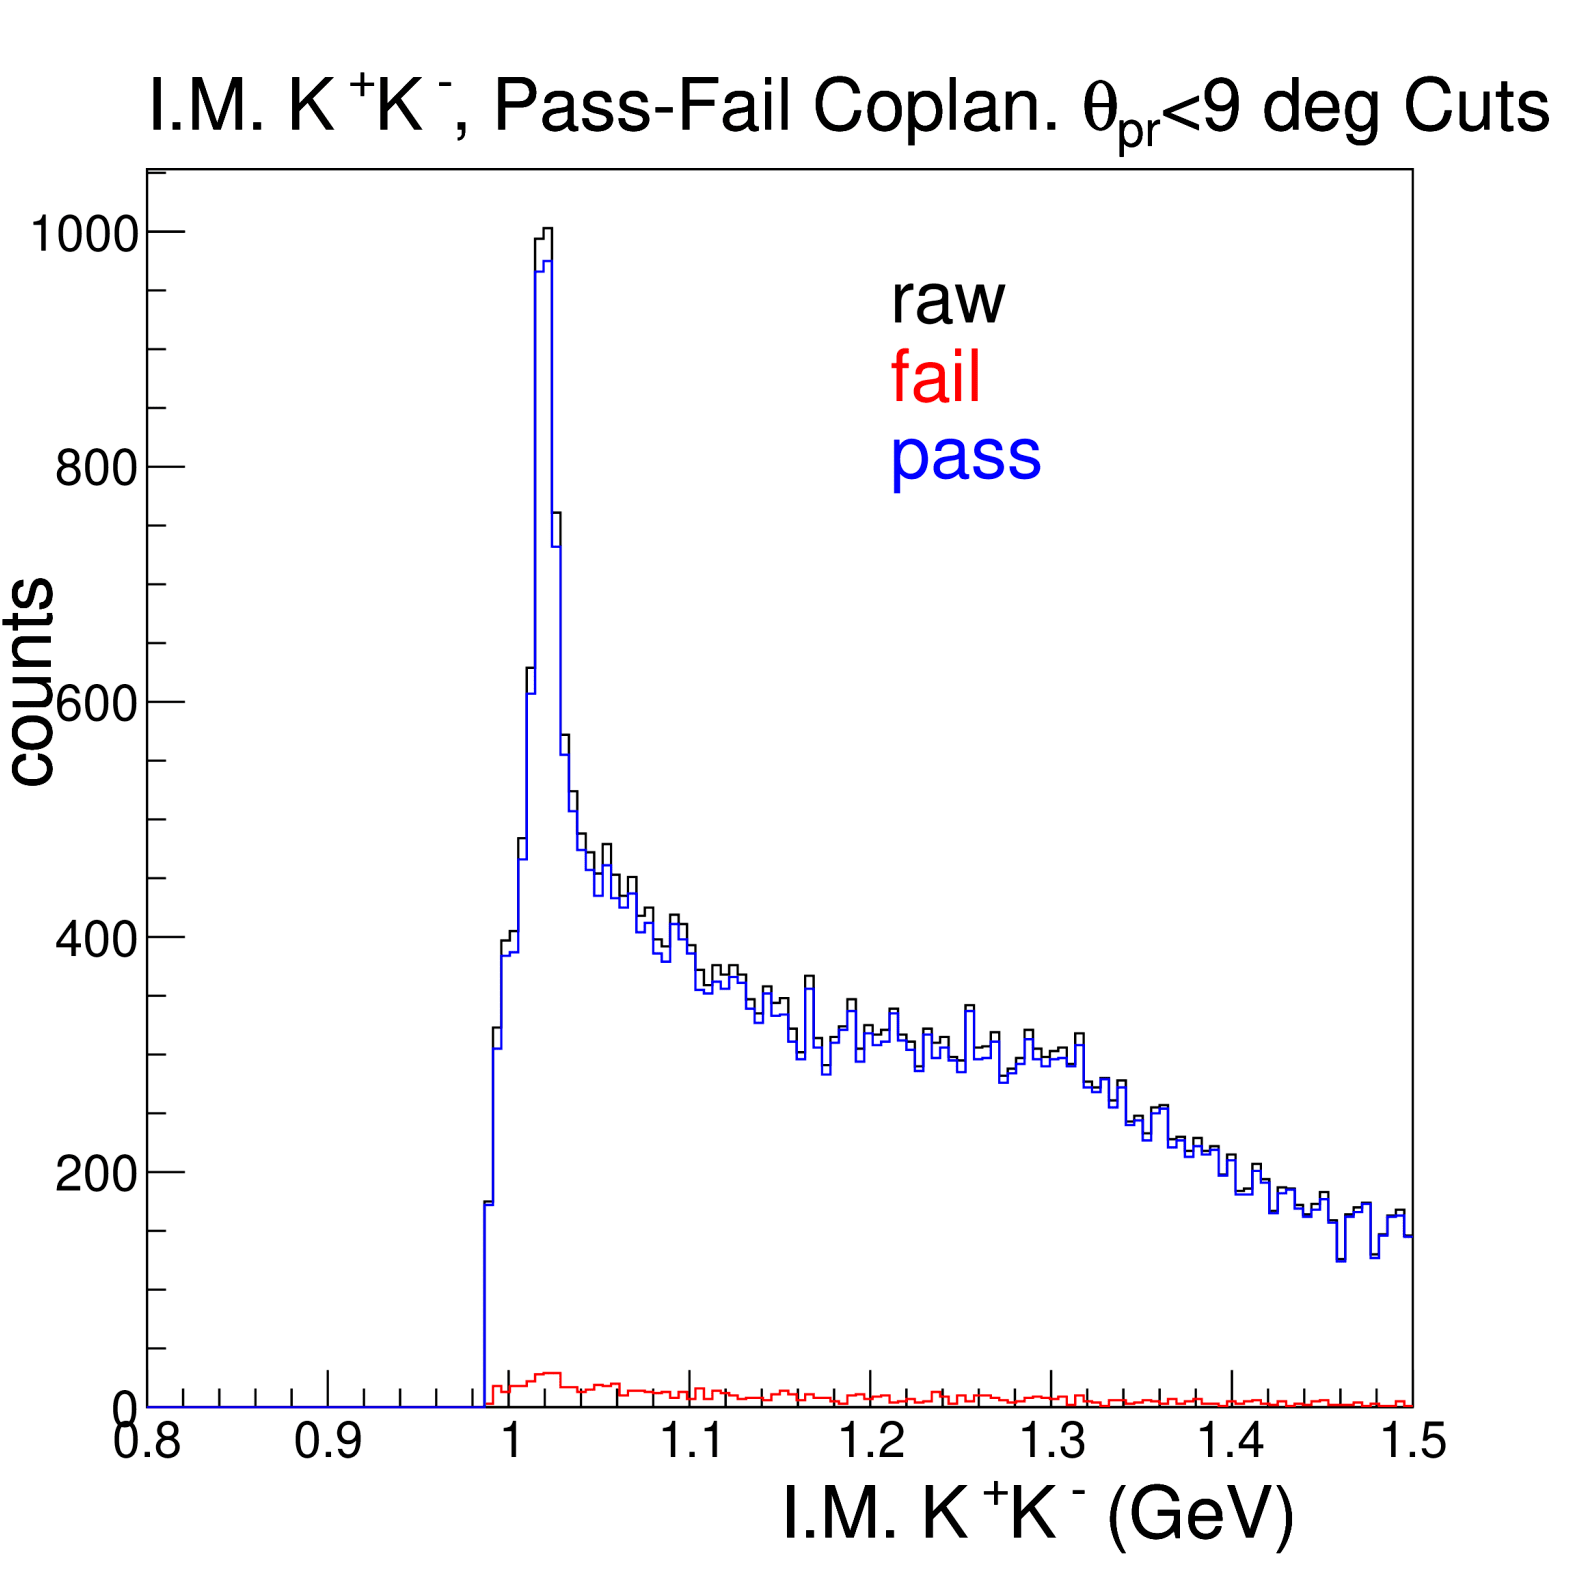
\includegraphics[width=0.94\textwidth]{brandon_figs/35b.png}
        \caption{Brandon 3.35b}
    \end{figure}
    \column{0.5\textwidth}
    \begin{figure}
        \centering
        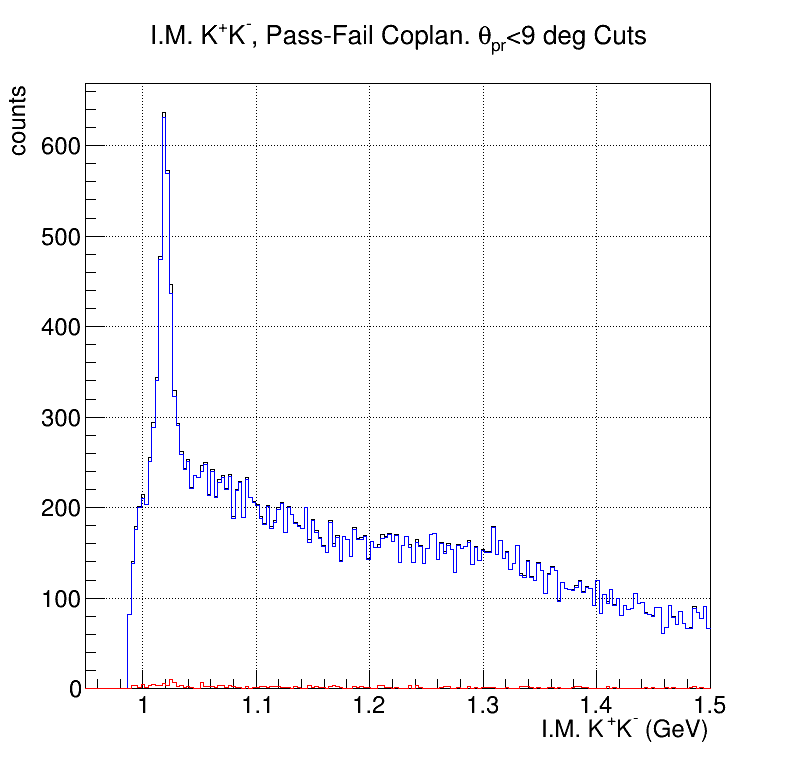
\includegraphics[width=0.97\textwidth]{pdfs/35b.png}
        \caption{My Reproduction}
    \end{figure}
    \end{columns}
\end{frame}

\begin{frame}{Coplanarity Cuts \hfill Skim4 FD}
\vspace*{-0.6cm}
    \begin{columns}
    \column{0.5\textwidth}
    \begin{figure}
        \centering
        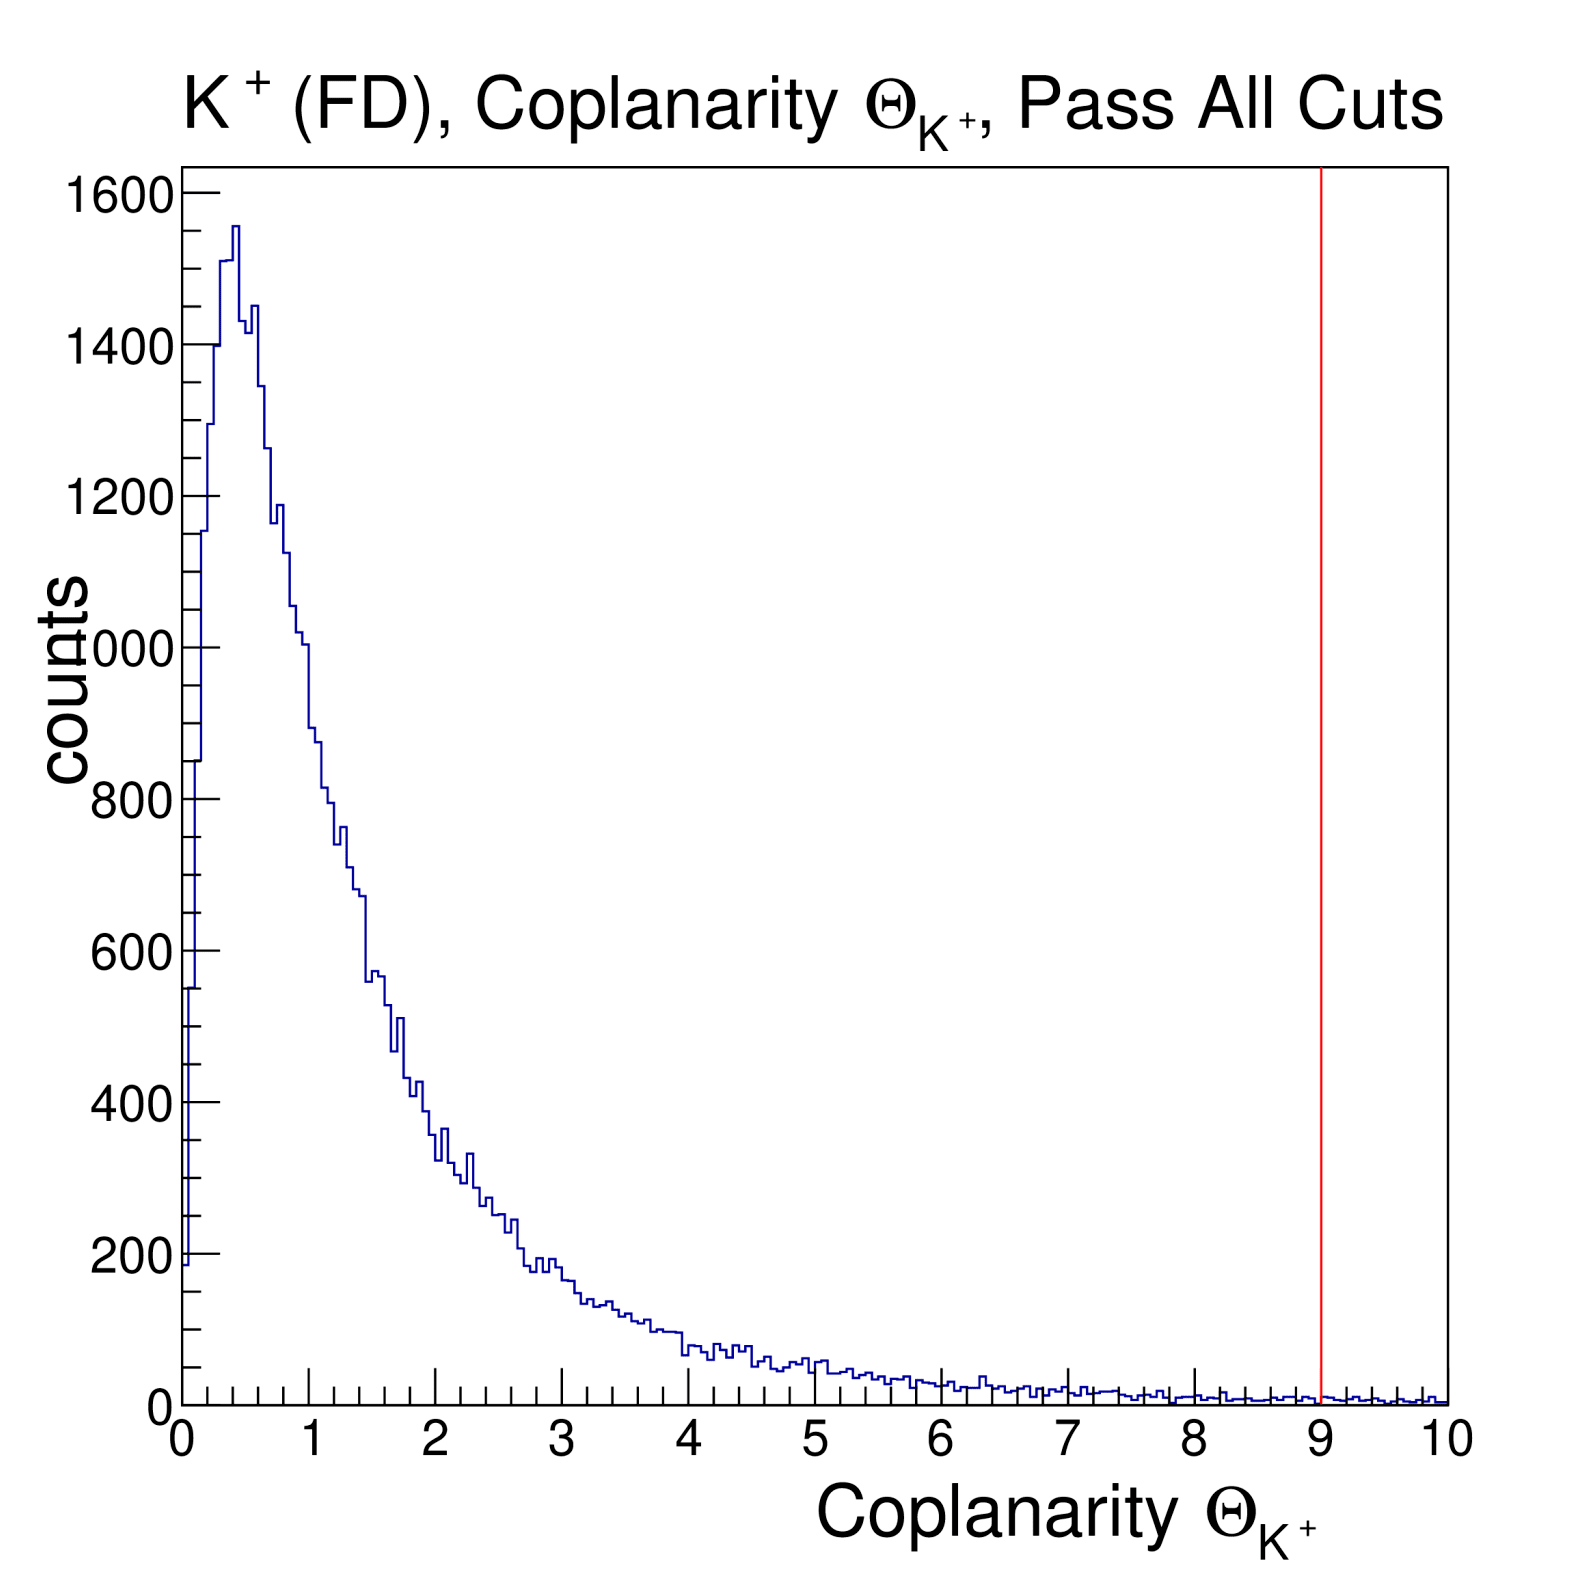
\includegraphics[width=0.94\textwidth]{brandon_figs/35c.png}
        \caption{Brandon 3.35c}
    \end{figure}
    \column{0.5\textwidth}
    \begin{figure}
        \centering
        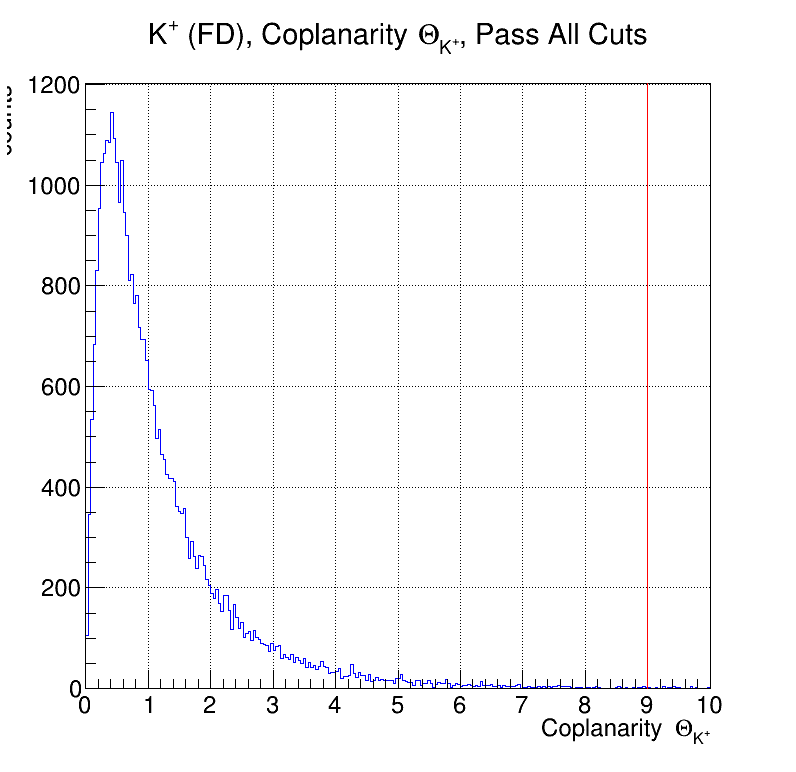
\includegraphics[width=0.97\textwidth]{pdfs/35c.png}
        \caption{My Reproduction}
    \end{figure}
    \end{columns}
\end{frame}

\begin{frame}{Coplanarity Cuts \hfill Skim4 FD}
\vspace*{-0.6cm}
    \begin{columns}
    \column{0.5\textwidth}
    \begin{figure}
        \centering
        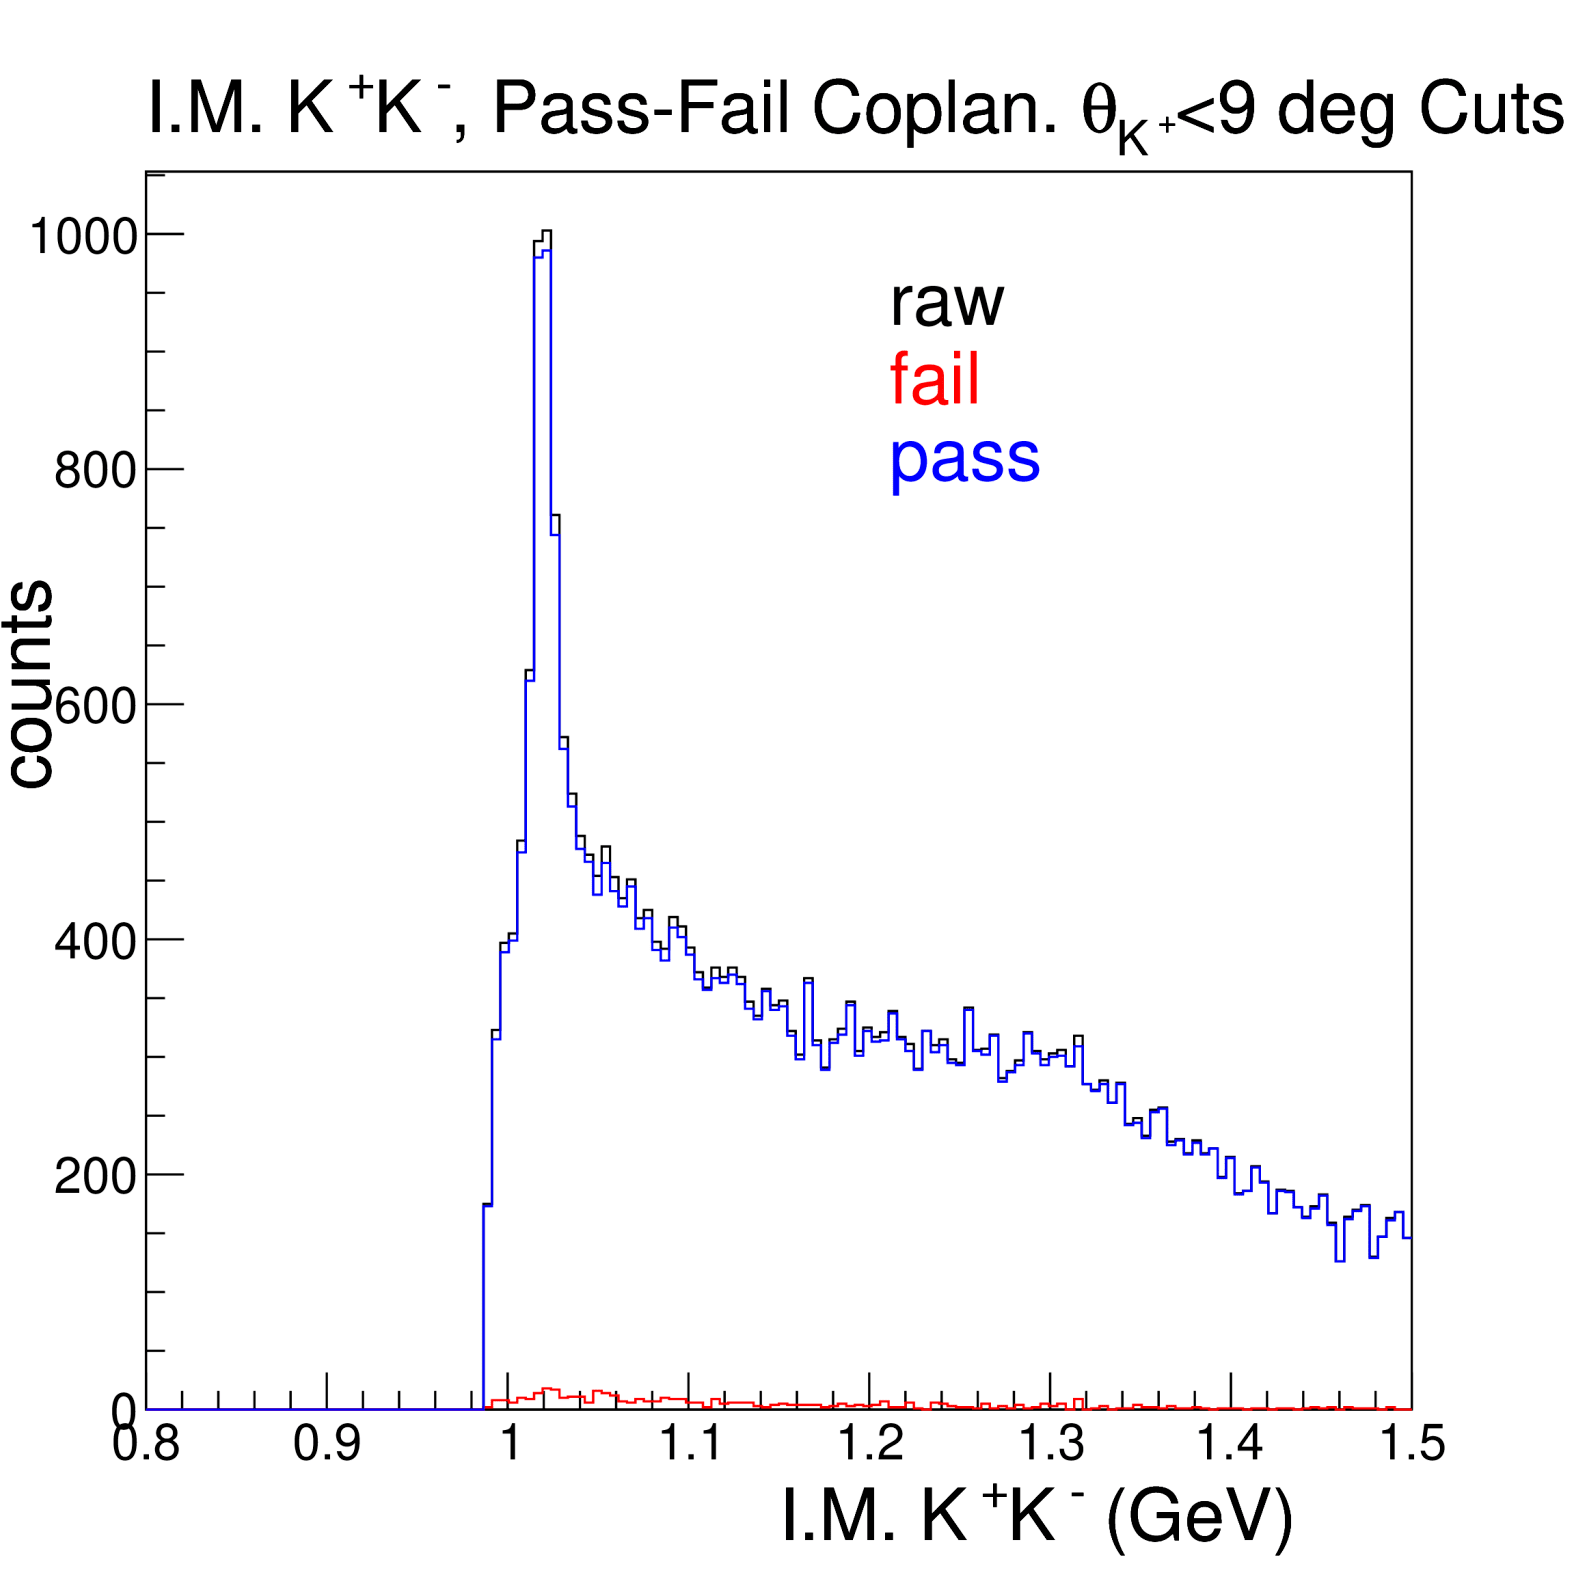
\includegraphics[width=0.94\textwidth]{brandon_figs/35d.png}
        \caption{Brandon 3.35d}
    \end{figure}
    \column{0.5\textwidth}
    \begin{figure}
        \centering
        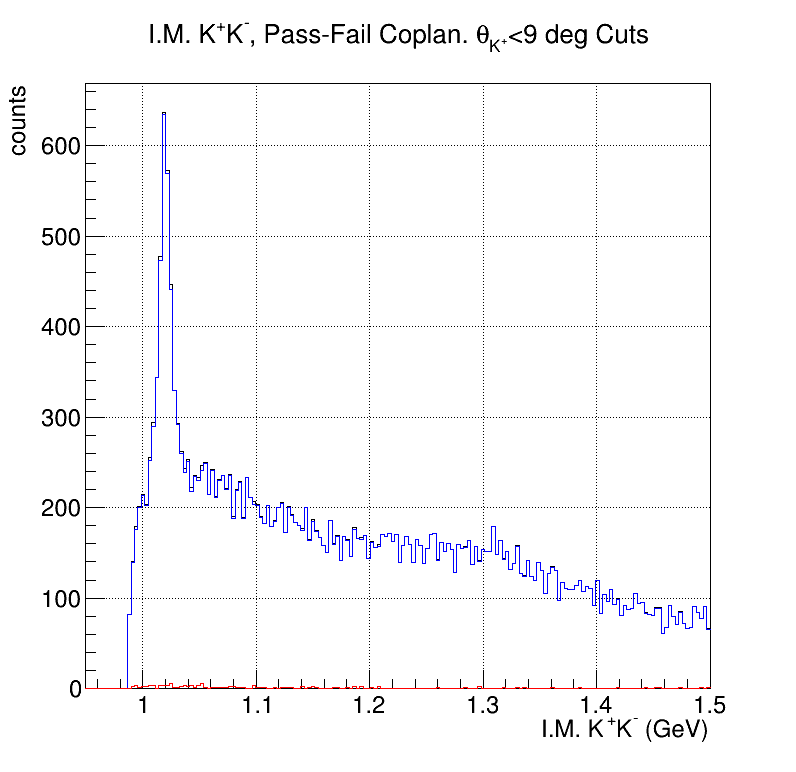
\includegraphics[width=0.97\textwidth]{pdfs/35d.png}
        \caption{My Reproduction}
    \end{figure}
    \end{columns}
\end{frame}

\begin{frame}{Coplanarity Cuts \hfill Skim4 FD}
\vspace*{-0.6cm}
    \begin{columns}
    \column{0.5\textwidth}
    \begin{figure}
        \centering
        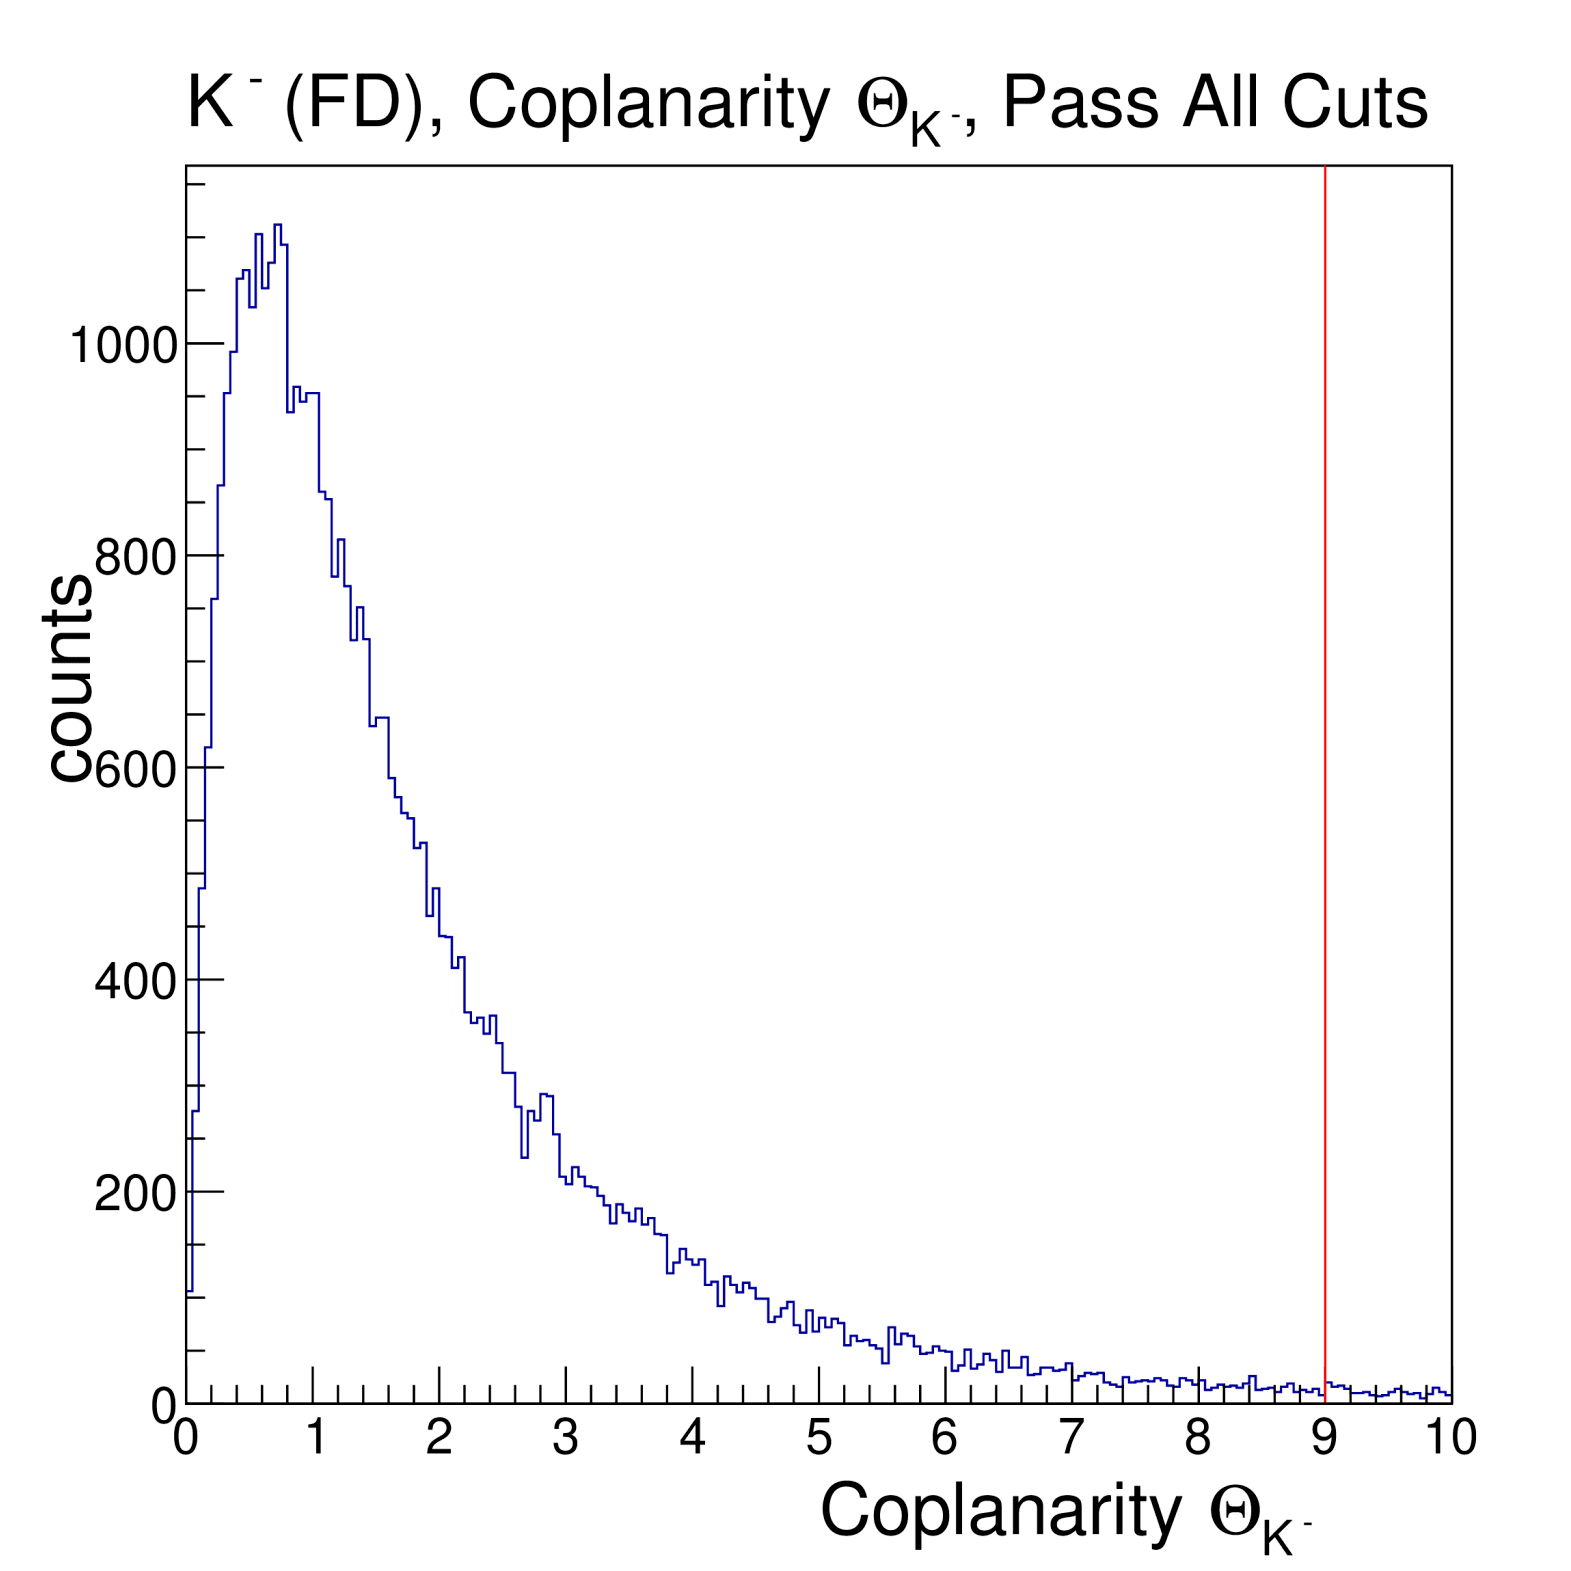
\includegraphics[width=0.94\textwidth]{brandon_figs/35e.png}
        \caption{Brandon 3.35e}
    \end{figure}
    \column{0.5\textwidth}
    \begin{figure}
        \centering
        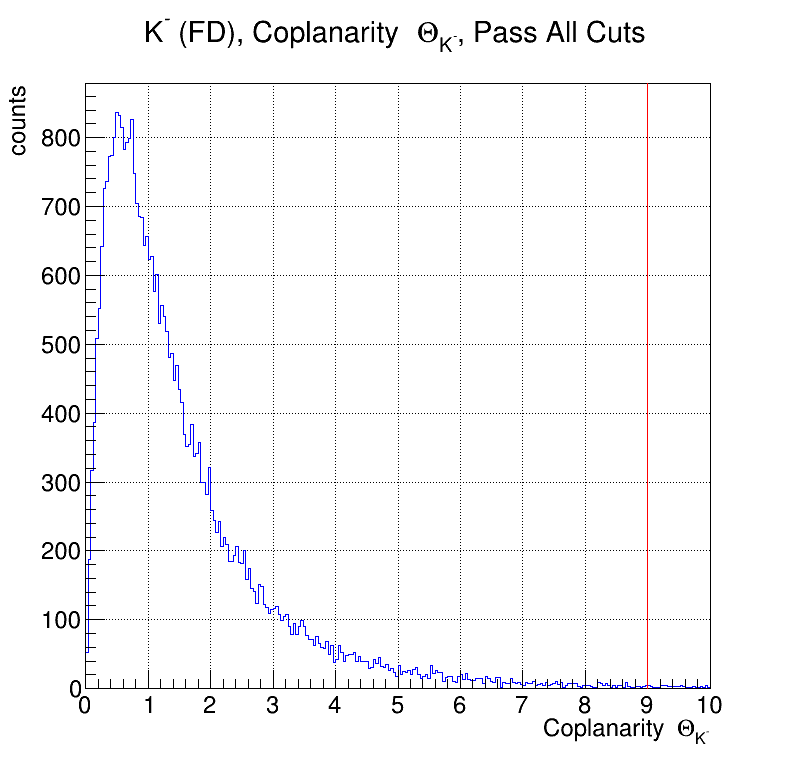
\includegraphics[width=0.97\textwidth]{pdfs/35e.png}
        \caption{My Reproduction}
    \end{figure}
    \end{columns}
\end{frame}

\begin{frame}{Coplanarity Cuts \hfill Skim4 FD}
\vspace*{-0.6cm}
    \begin{columns}
    \column{0.5\textwidth}
    \begin{figure}
        \centering
        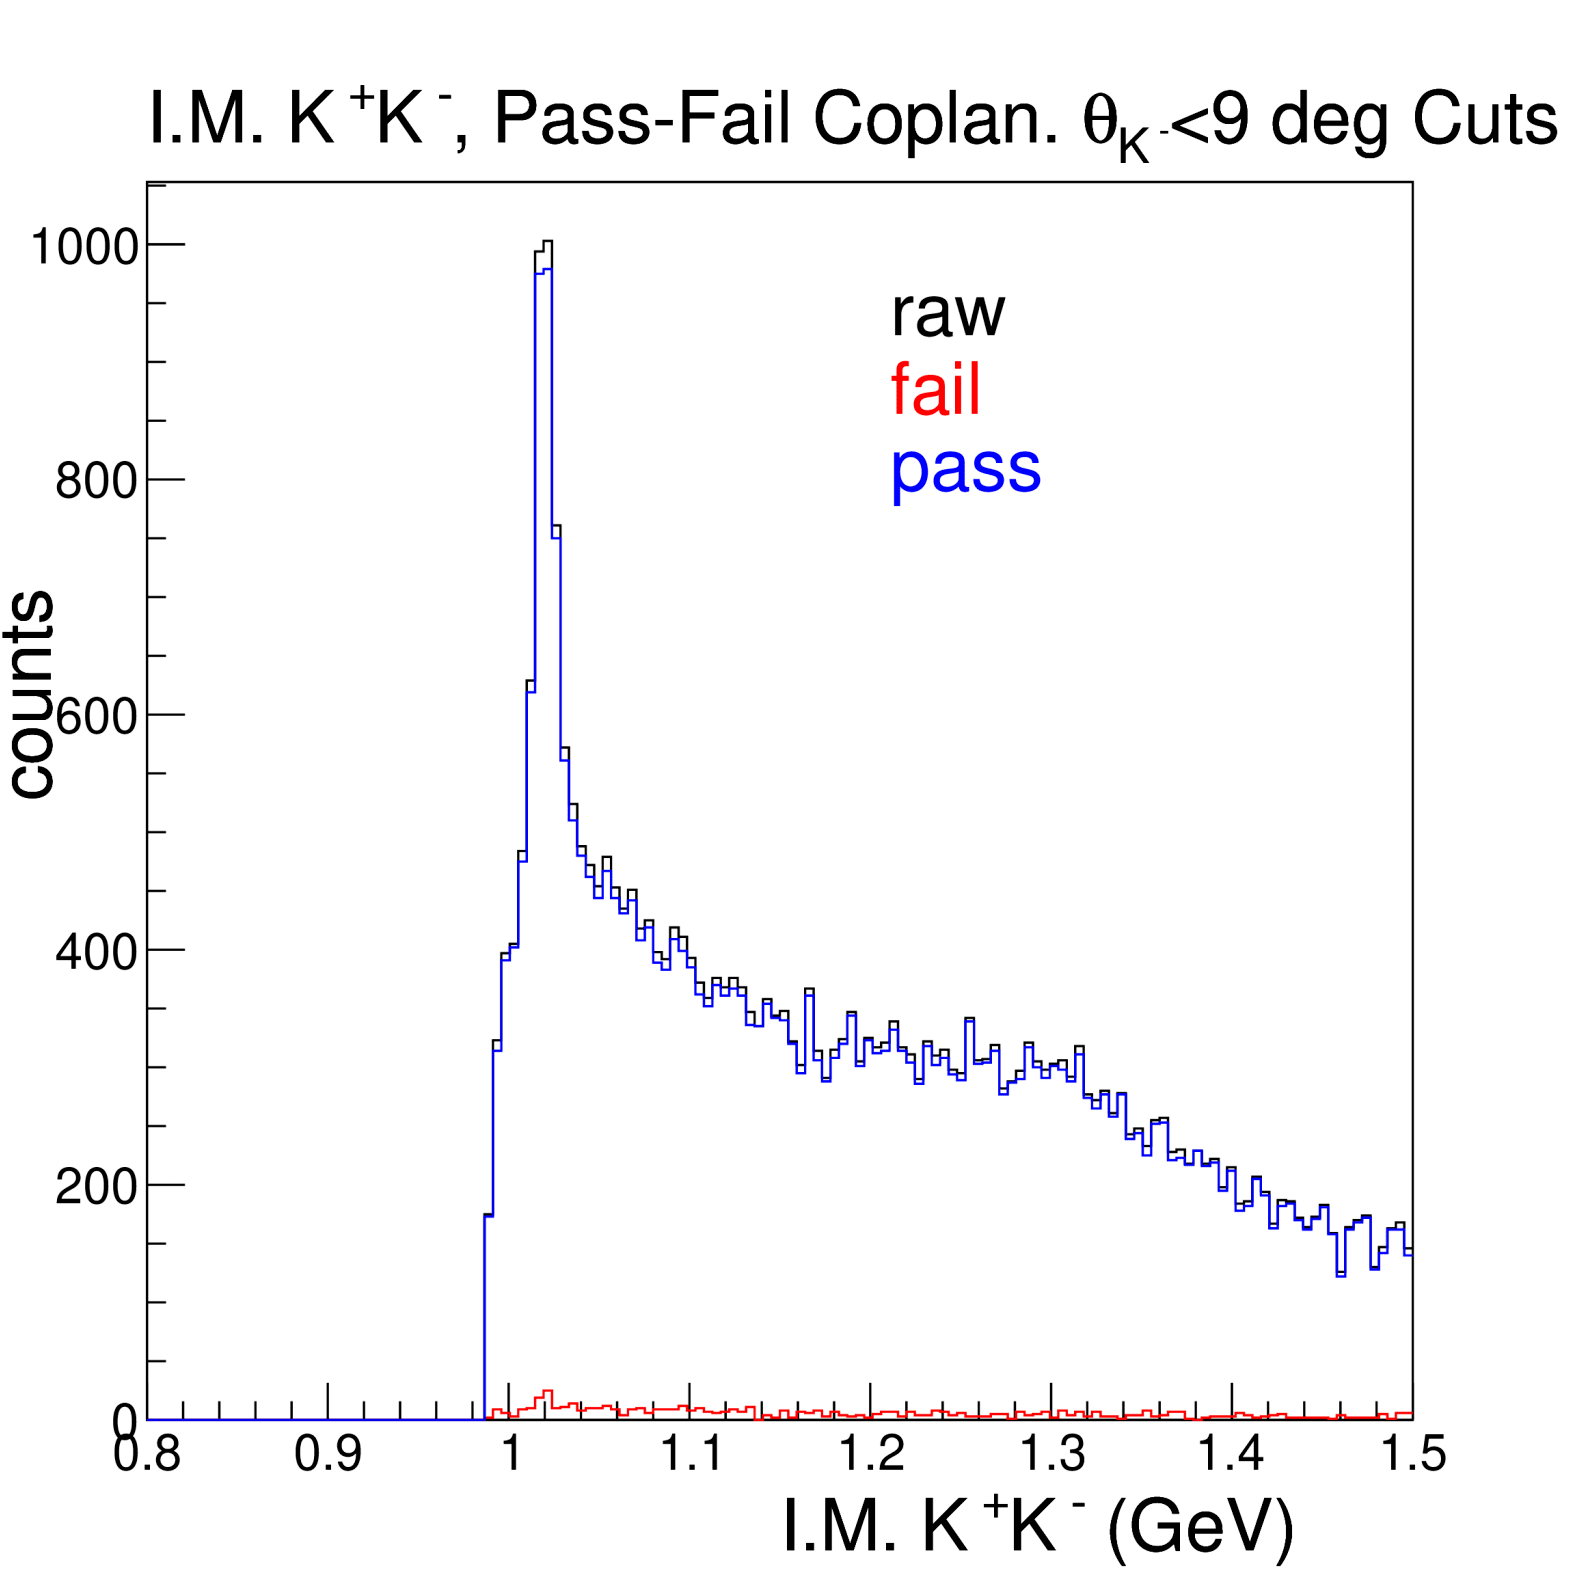
\includegraphics[width=0.94\textwidth]{brandon_figs/35f.png}
        \caption{Brandon 3.35f}
    \end{figure}
    \column{0.5\textwidth}
    \begin{figure}
        \centering
        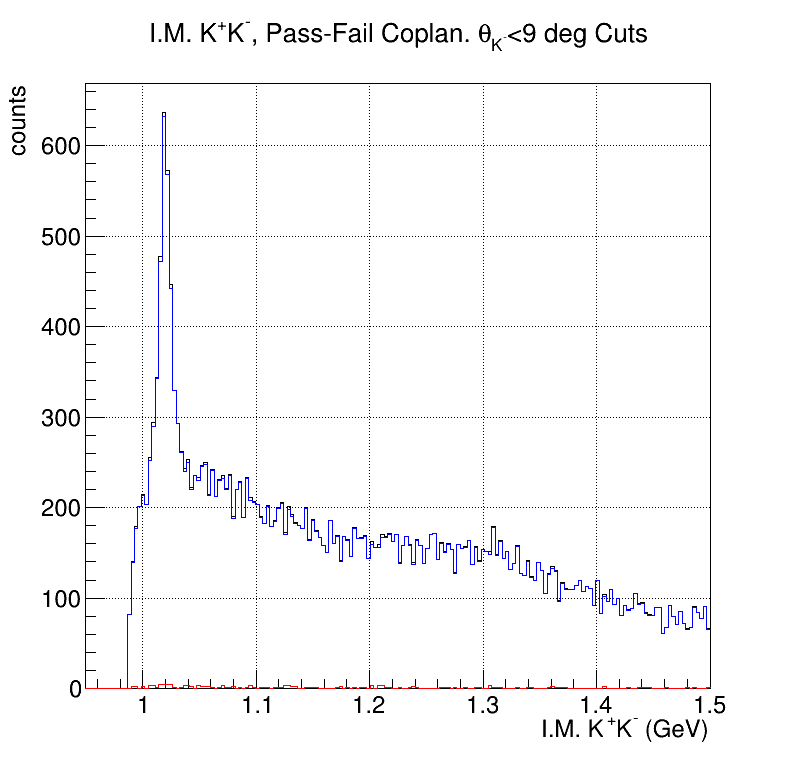
\includegraphics[width=0.97\textwidth]{pdfs/35f.png}
        \caption{My Reproduction}
    \end{figure}
    \end{columns}
\end{frame}

\begin{frame}{Coplanarity Cuts \hfill Skim4 FD}
\vspace*{-0.6cm}
    \begin{columns}
    \column{0.5\textwidth}
    \begin{figure}
        \centering
        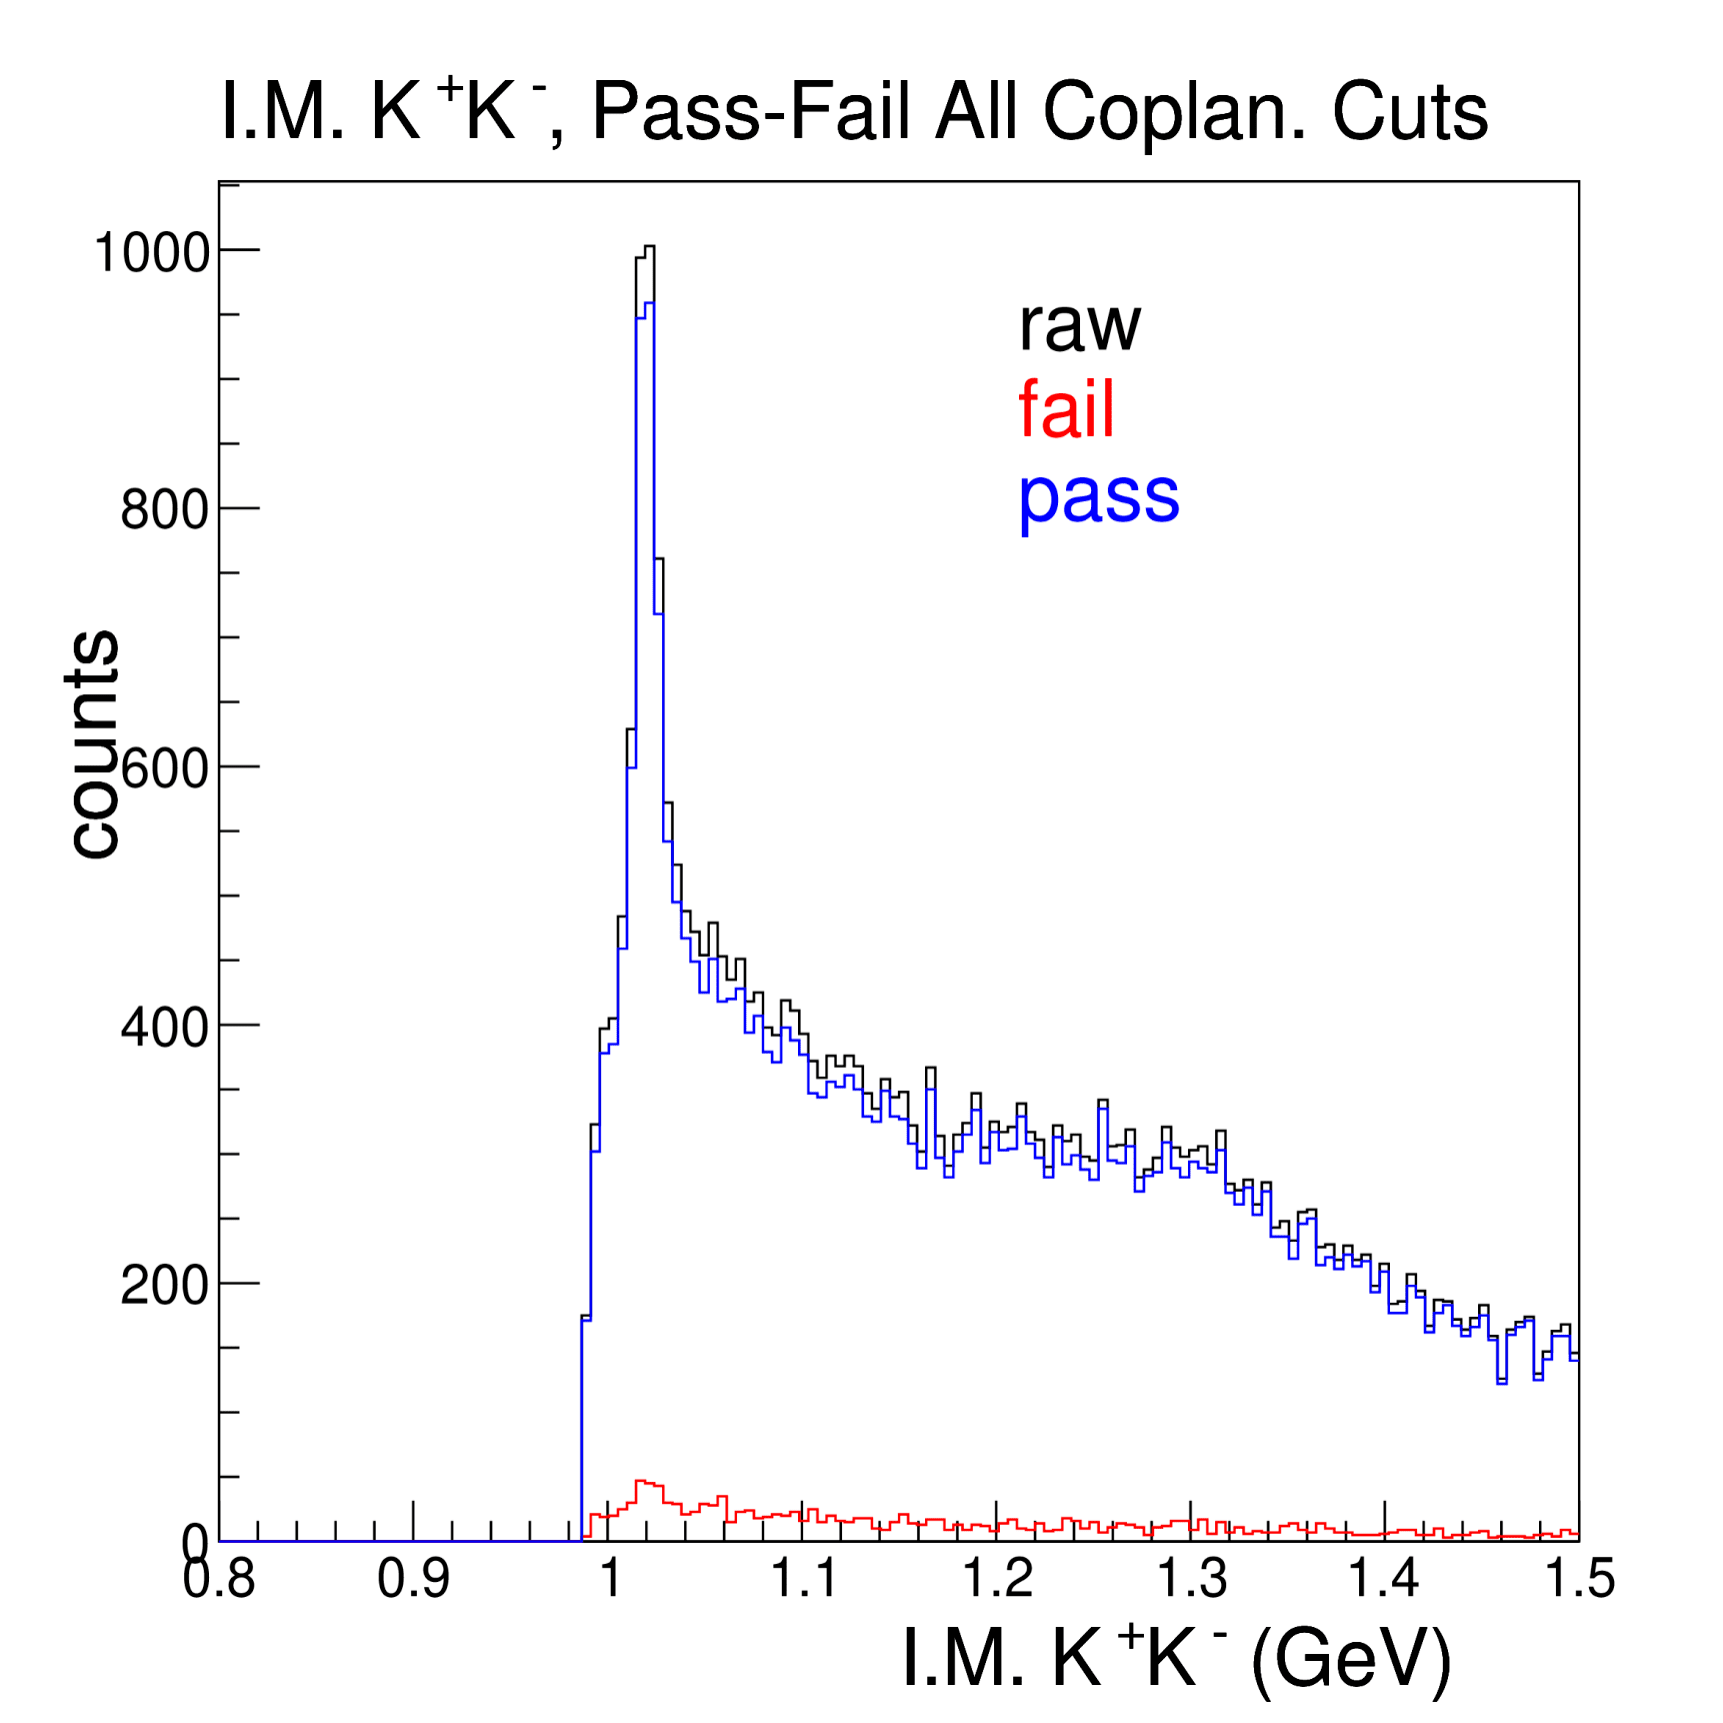
\includegraphics[width=0.94\textwidth]{brandon_figs/36.png}
        \caption{Brandon 3.36}
    \end{figure}
    \column{0.5\textwidth}
    \begin{figure}
        \centering
        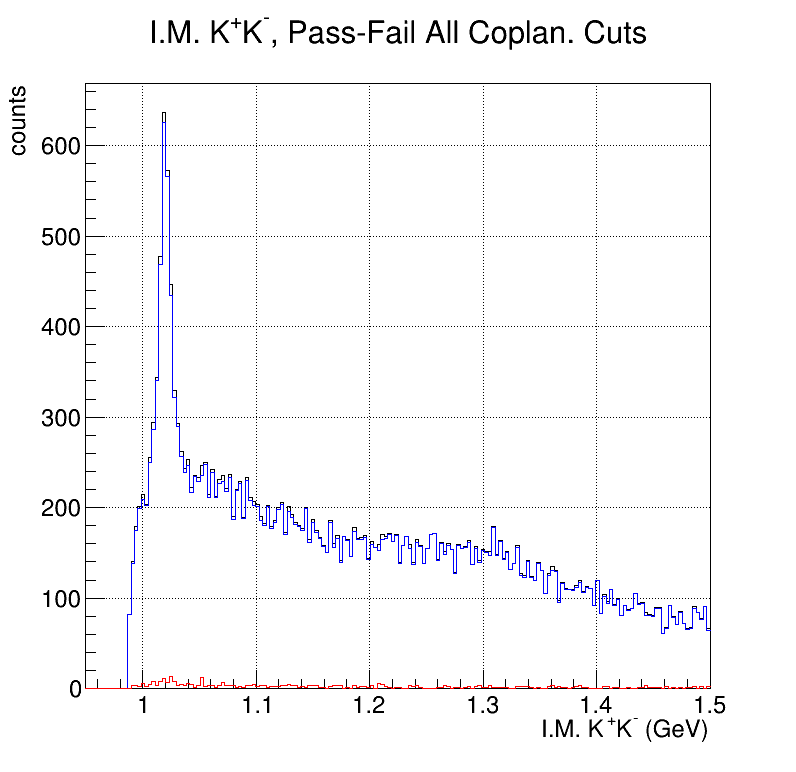
\includegraphics[width=0.97\textwidth]{pdfs/36.png}
        \caption{My Reproduction}
    \end{figure}
    \end{columns}
\end{frame}

\begin{frame}{Removal of Resonant Structures from $\Lambda$ 1520 \& 1820  \hfill Skim4 FD}
\vspace*{-0.6cm}
    \begin{columns}
    \column{0.5\textwidth}
    \begin{figure}
        \centering
        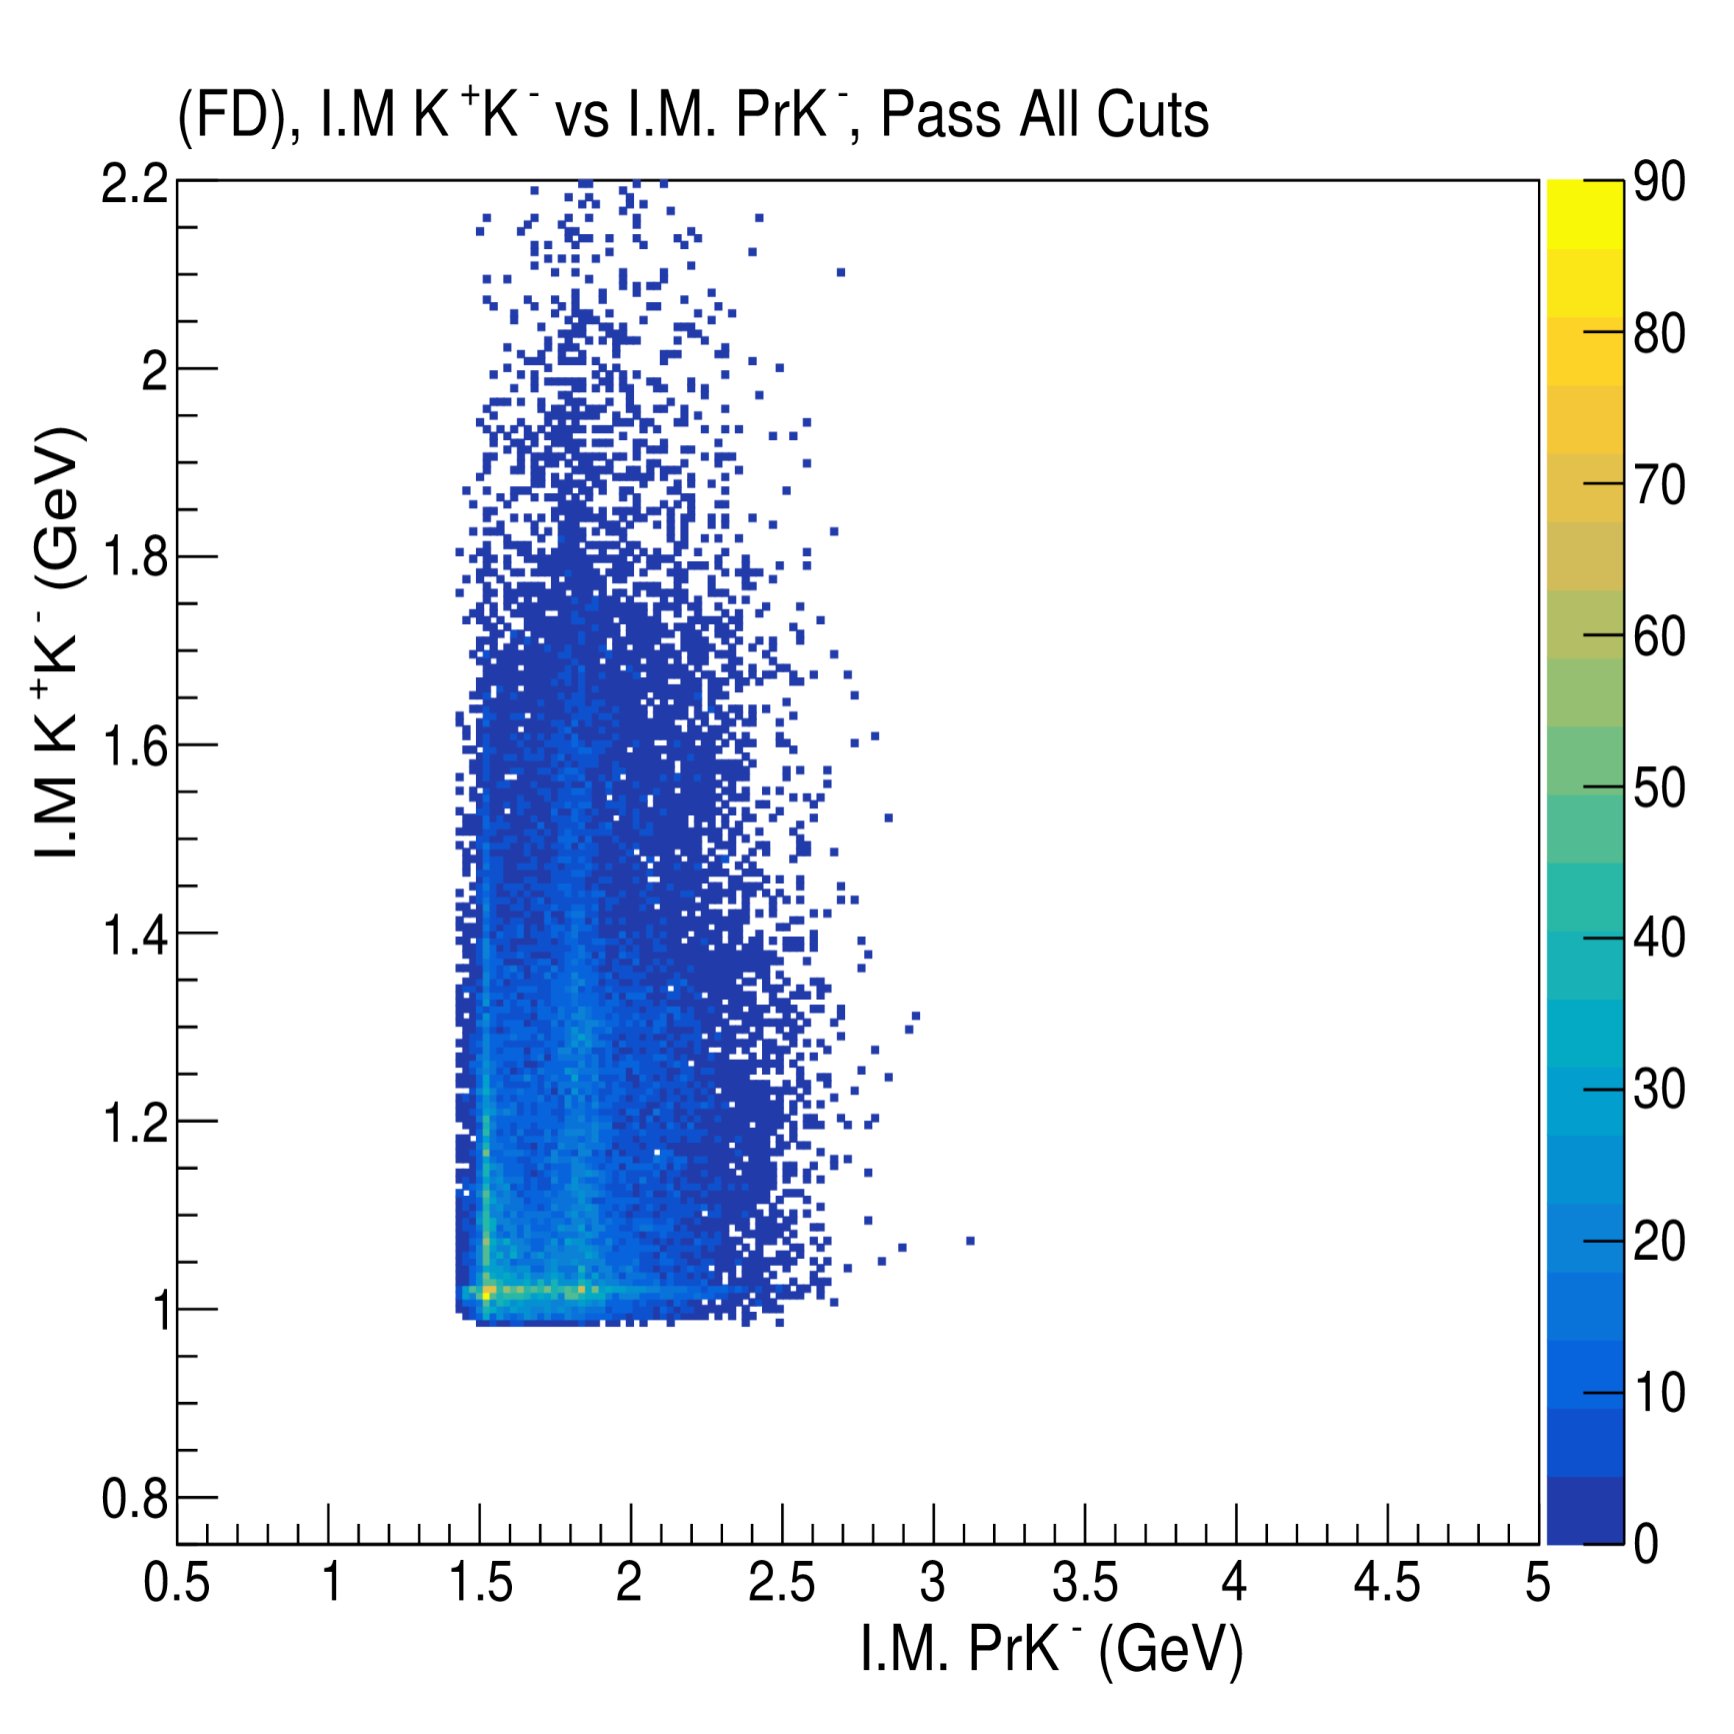
\includegraphics[width=0.94\textwidth]{brandon_figs/33.png}
        \caption{Brandon 3.33}
    \end{figure}
    \column{0.5\textwidth}
    \begin{figure}
        \centering
        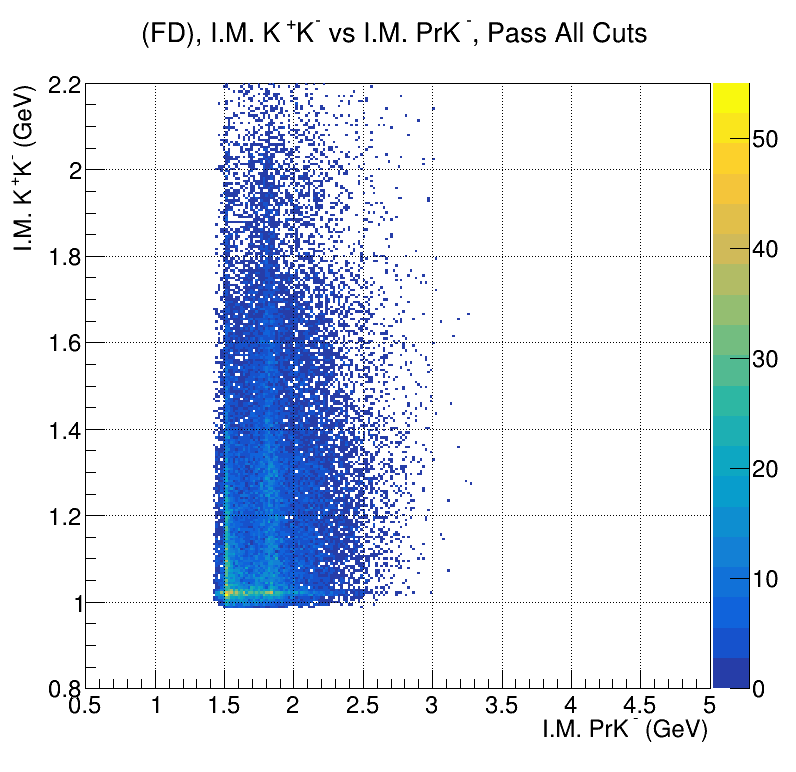
\includegraphics[width=0.97\textwidth]{pdfs/33.png}
        \caption{My Reproduction}
    \end{figure}
    \end{columns}
\end{frame}

\begin{frame}{Removal of Resonant Structures from $\Lambda$ 1520 \& 1820  \hfill Skim4 FD}
\vspace*{-0.6cm}
    \begin{columns}
    \column{0.5\textwidth}
    \begin{figure}
        \centering
        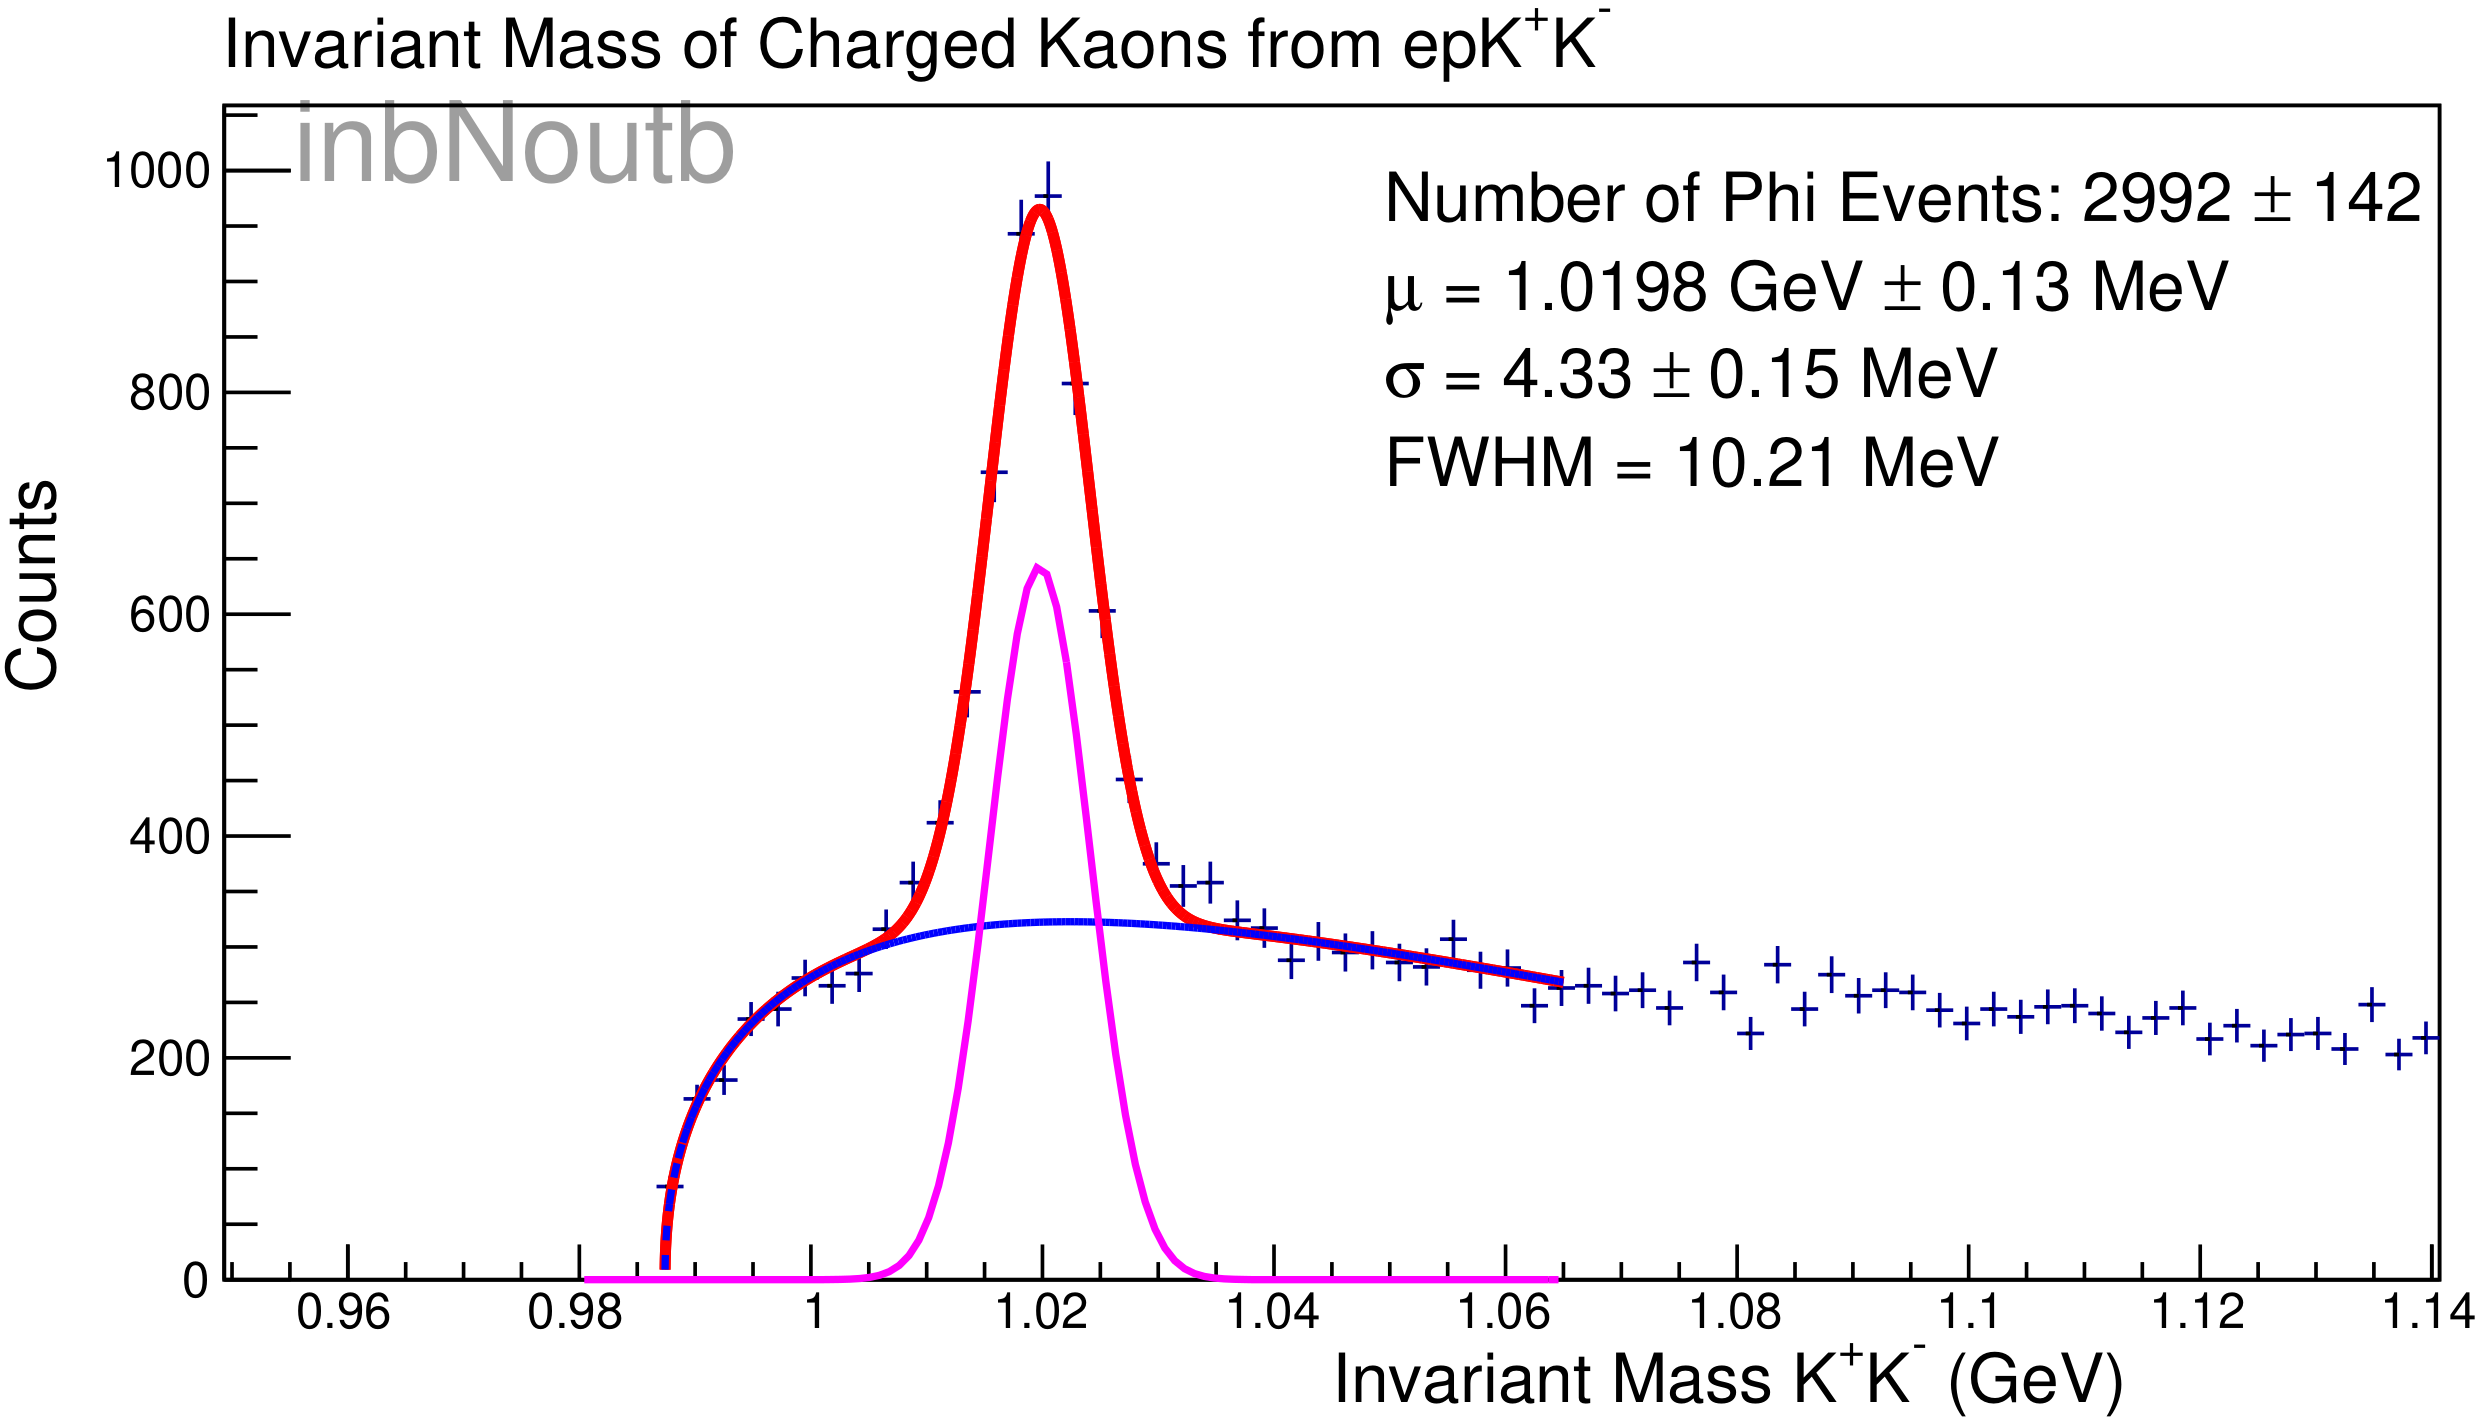
\includegraphics[width=0.94\textwidth]{brandon_figs/38.png}
        \caption{Brandon 3.38}
    \end{figure}
    \column{0.5\textwidth}
    \begin{figure}
        \centering
        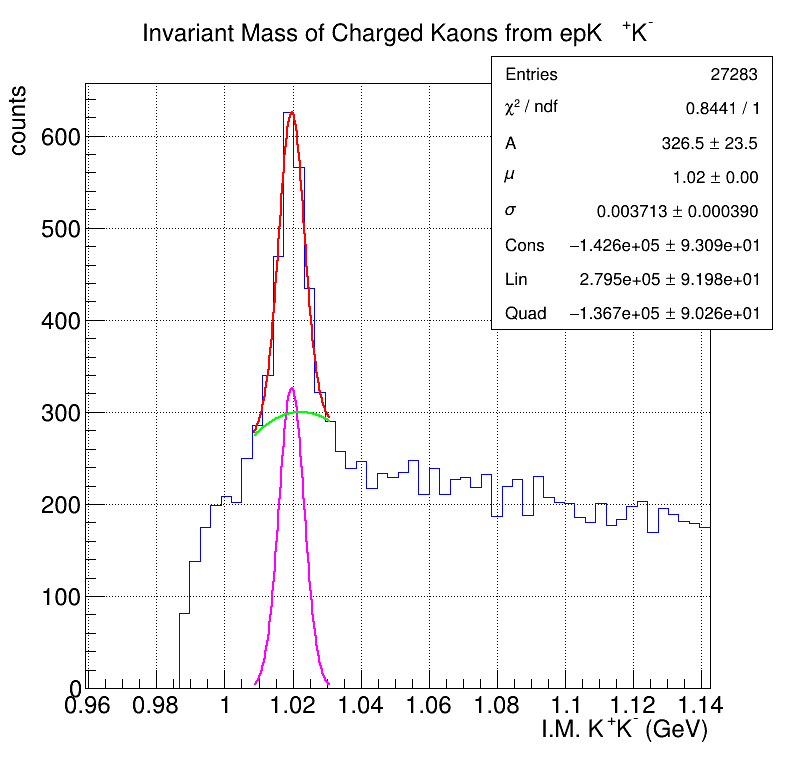
\includegraphics[width=0.97\textwidth]{pdfs/38.png}
        \caption{My Reproduction}
    \end{figure}
    \end{columns}
\end{frame}

\begin{frame}{Removal of Resonant Structures from $\Lambda$ 1520 \& 1820  \hfill Skim4 FD}
\vspace*{-0.6cm}
    \begin{columns}
    \column{0.5\textwidth}
    \begin{figure}
        \centering
        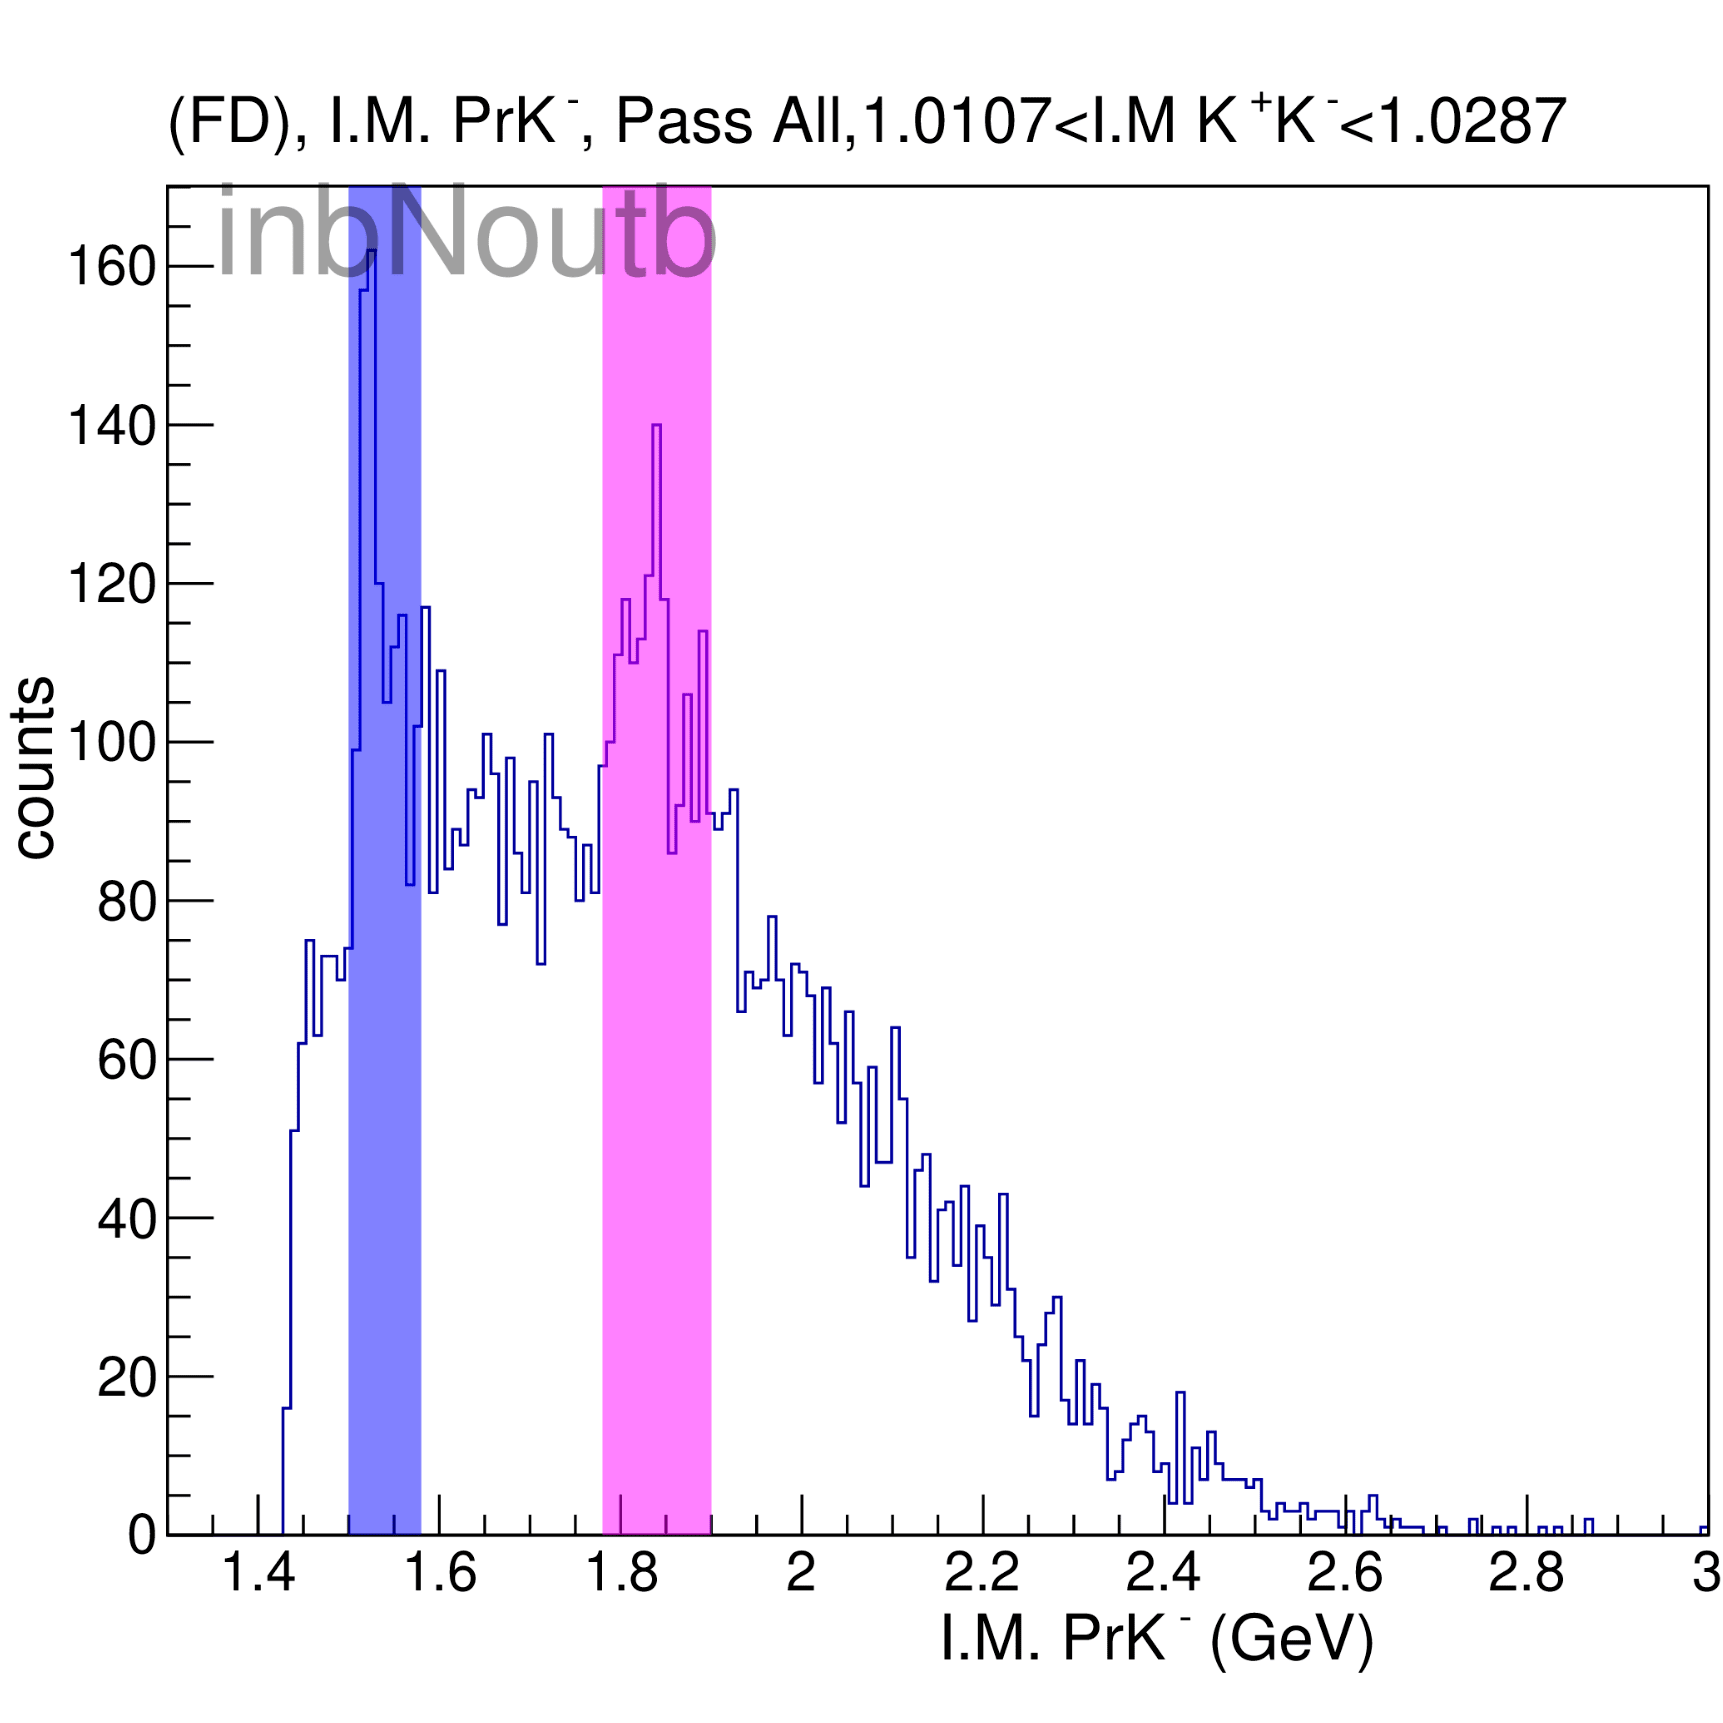
\includegraphics[width=0.94\textwidth]{brandon_figs/37.png}
        \caption{Brandon 3.37}
    \end{figure}
    \column{0.5\textwidth}
    \begin{figure}
        \centering
        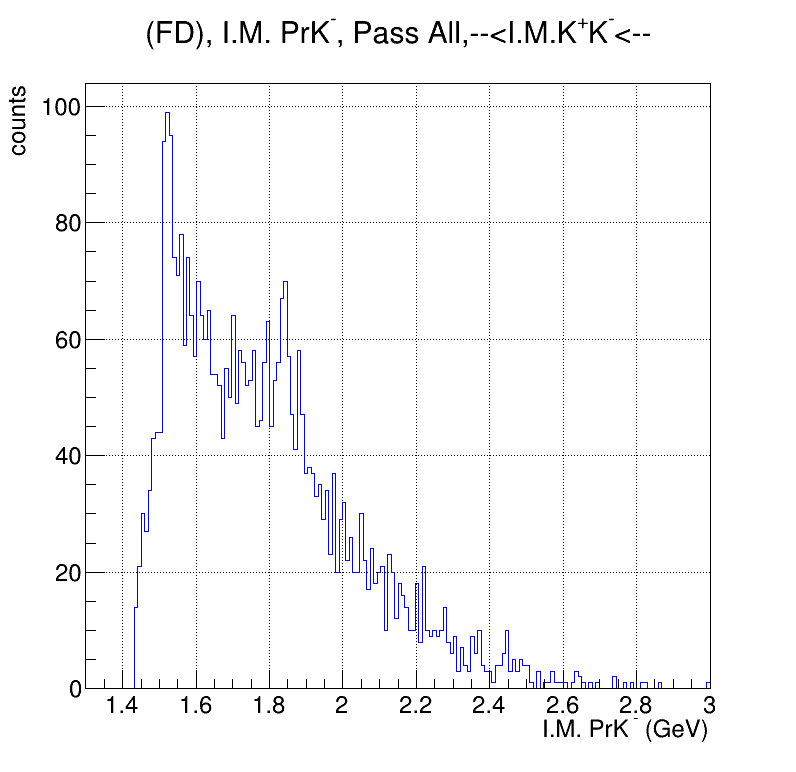
\includegraphics[width=0.97\textwidth]{pdfs/37.png}
        \caption{My Reproduction}
    \end{figure}
    \end{columns}
\end{frame}


\begin{frame}{Diagnostics}
\centering
    \Huge{Phase space, Q\textsuperscript{2}, W, \& x\textsubscript{B} measurements}
\end{frame}

\begin{frame}{Phase Space  \hfill Skim4 FD}
\vspace*{-0.6cm}
    \begin{columns}
    \column{0.5\textwidth}
    \begin{figure}
        \centering
        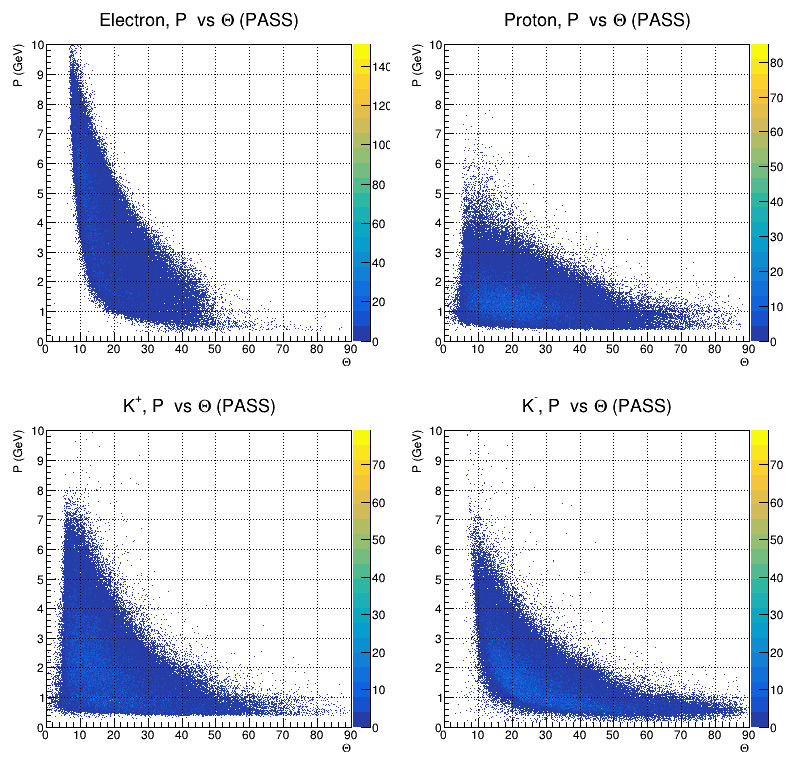
\includegraphics[width=0.97\textwidth]{pdfs/hists/PASS/ThetaP.png}
        \caption{No Cuts}
    \end{figure}
    \column{0.5\textwidth}
    \begin{figure}
        \centering
        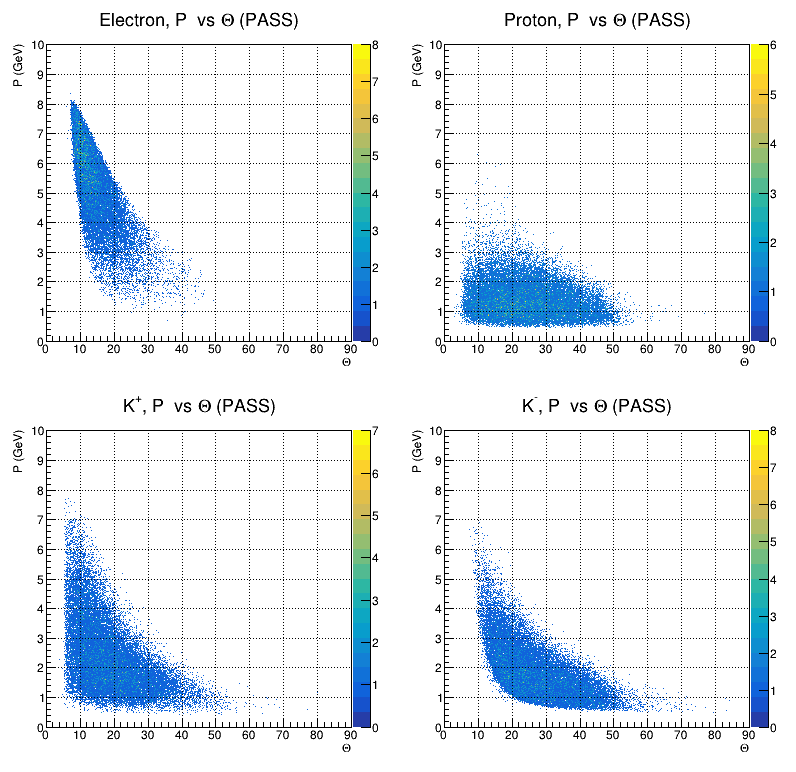
\includegraphics[width=0.97\textwidth]{pdfs/all_cuts/PASS/ThetaP.png}
        \caption{All Cuts}
    \end{figure}
    \end{columns}
\end{frame}

\begin{frame}{Phase Space  \hfill Skim4 FD}
\vspace*{-0.6cm}
    \begin{columns}
    \column{0.5\textwidth}
    \begin{figure}
        \centering
        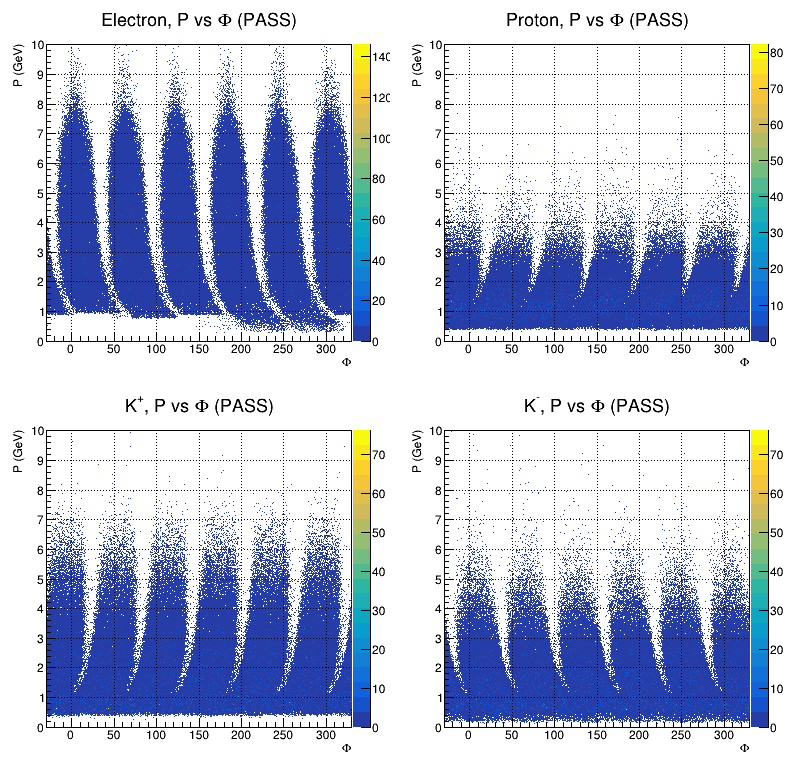
\includegraphics[width=0.97\textwidth]{pdfs/hists/PASS/PhiP.png}
        \caption{No Cuts}
    \end{figure}
    \column{0.5\textwidth}
    \begin{figure}
        \centering
        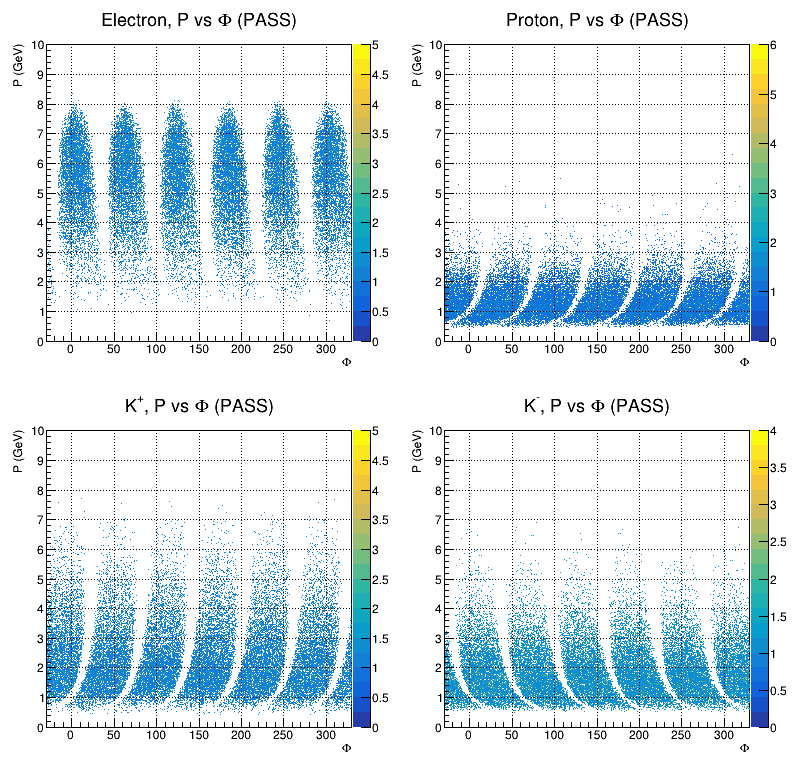
\includegraphics[width=0.97\textwidth]{pdfs/all_cuts/PASS/PhiP.png}
        \caption{All Cuts}
    \end{figure}
    \end{columns}
\end{frame}

\begin{frame}{Phase Space  \hfill Skim4 FD}
\vspace*{-0.6cm}
    \begin{columns}
    \column{0.5\textwidth}
    \begin{figure}
        \centering
        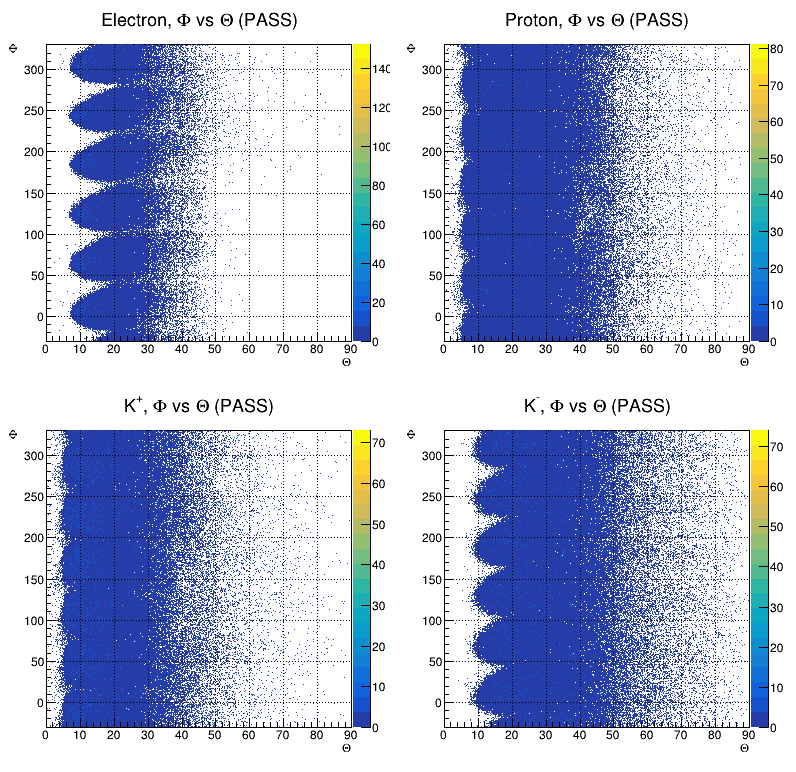
\includegraphics[width=0.97\textwidth]{pdfs/hists/PASS/ThetaPhi.png}
        \caption{No Cuts}
    \end{figure}
    \column{0.5\textwidth}
    \begin{figure}
        \centering
        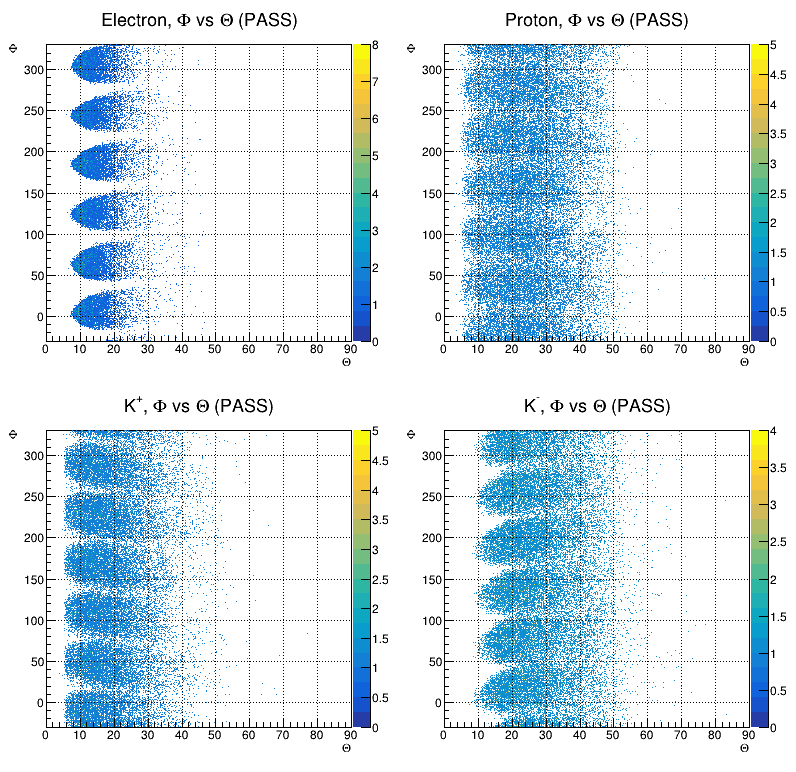
\includegraphics[width=0.97\textwidth]{pdfs/all_cuts/PASS/ThetaPhi.png}
        \caption{All Cuts}
    \end{figure}
    \end{columns}
\end{frame}

\begin{frame}{Q\textsuperscript{2} vs. W  \hfill Skim4 FD}
\vspace*{-0.6cm}
    \begin{columns}
    \column{0.5\textwidth}
    \begin{figure}
        \centering
        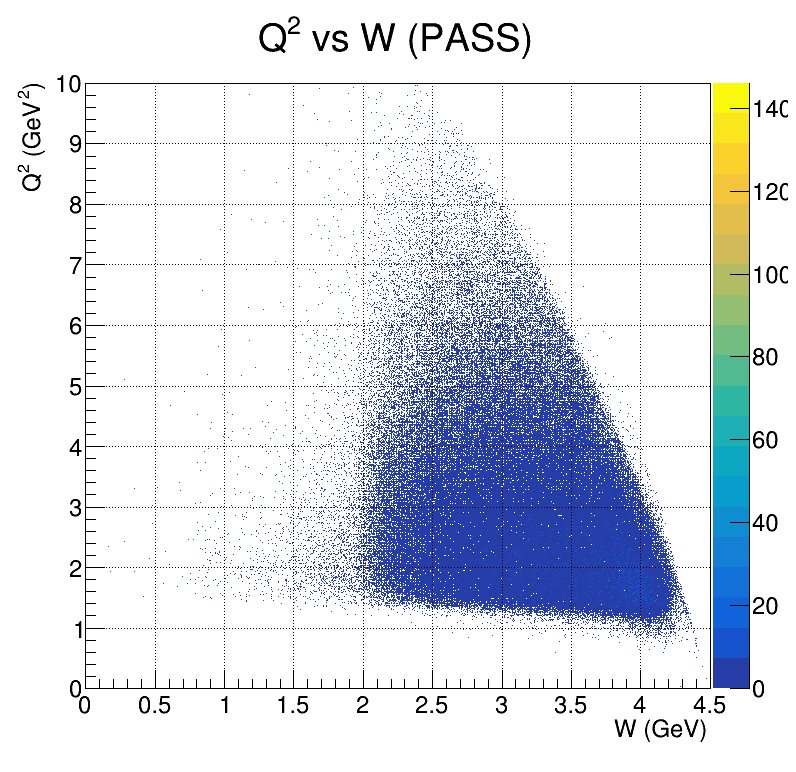
\includegraphics[width=0.97\textwidth]{pdfs/hists/PASS/q2w.png}
        \caption{No Cuts}
    \end{figure}
    \column{0.5\textwidth}
    \begin{figure}
        \centering
        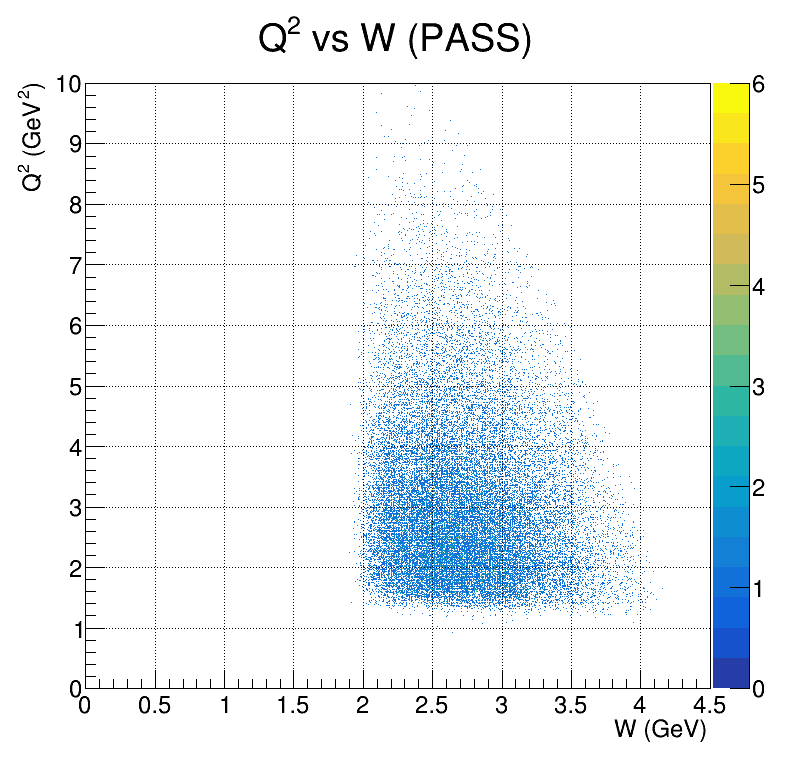
\includegraphics[width=0.97\textwidth]{pdfs/all_cuts/PASS/q2w.png}
        \caption{All Cuts}
    \end{figure}
    \end{columns}
\end{frame}

\begin{frame}{x\textsubscript{B}  \hfill Skim4 FD}
\vspace*{-0.6cm}
\begin{columns}
    \column{0.5\textwidth}
    \begin{figure}
        \centering
        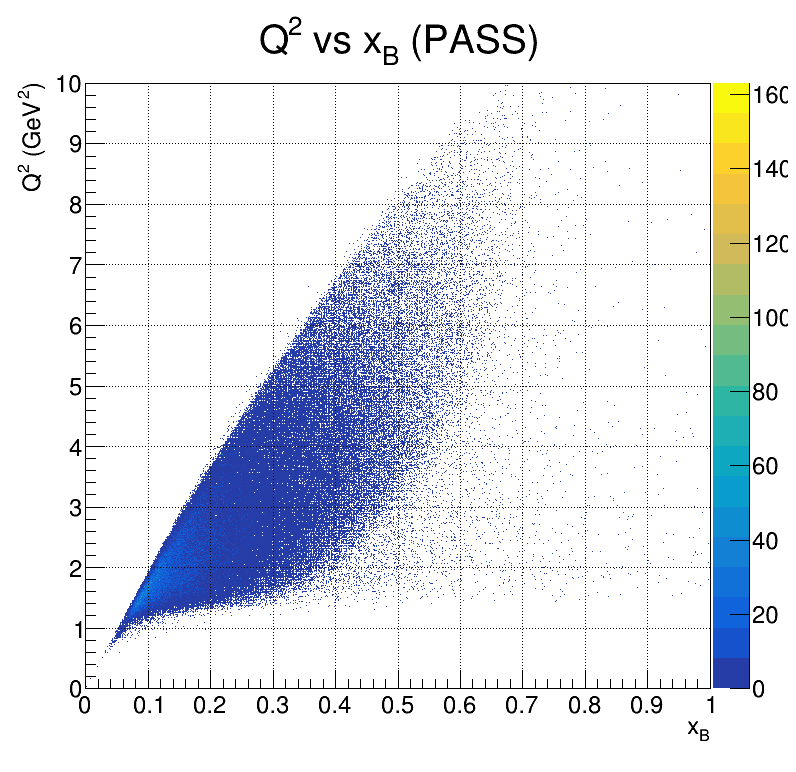
\includegraphics[width=0.97\textwidth]{pdfs/hists/PASS/q2Xb.png}
        \caption{No Cuts}
    \end{figure}
    \column{0.5\textwidth}
    \begin{figure}
        \centering
        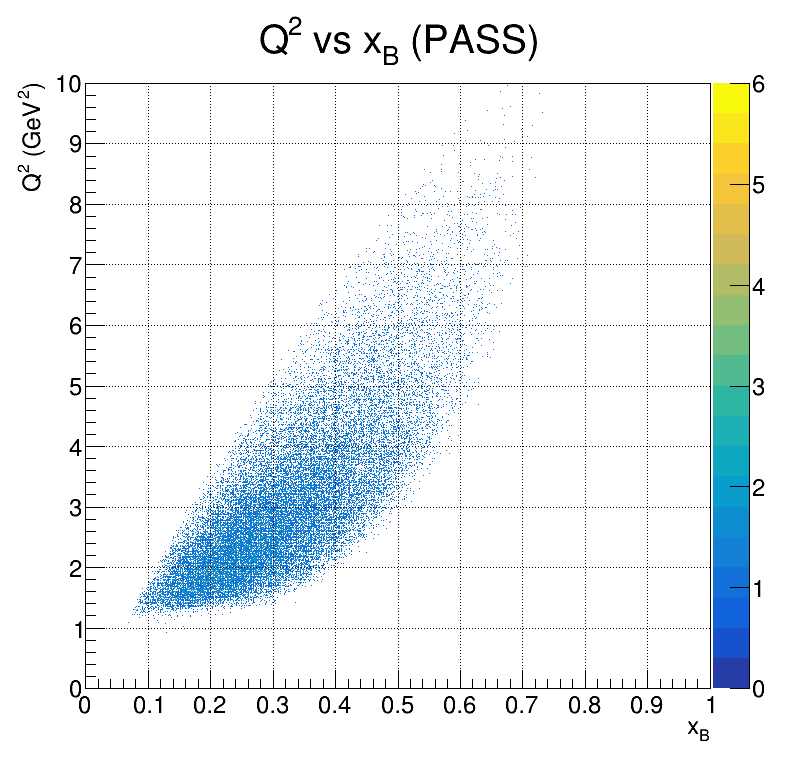
\includegraphics[width=0.97\textwidth]{pdfs/all_cuts/PASS/q2Xb.png}
        \caption{All Cuts}
    \end{figure}
    \end{columns}
\end{frame}


\end{document}


% \begin{frame}{Coplanarity Cuts \hfill Skim4 FD}
% \vspace*{-0.55cm}
%     \begin{columns}
%     \column{0.5\textwidth}
    
%     \column{0.5\textwidth}
%     \begin{figure}
%         \centering
%         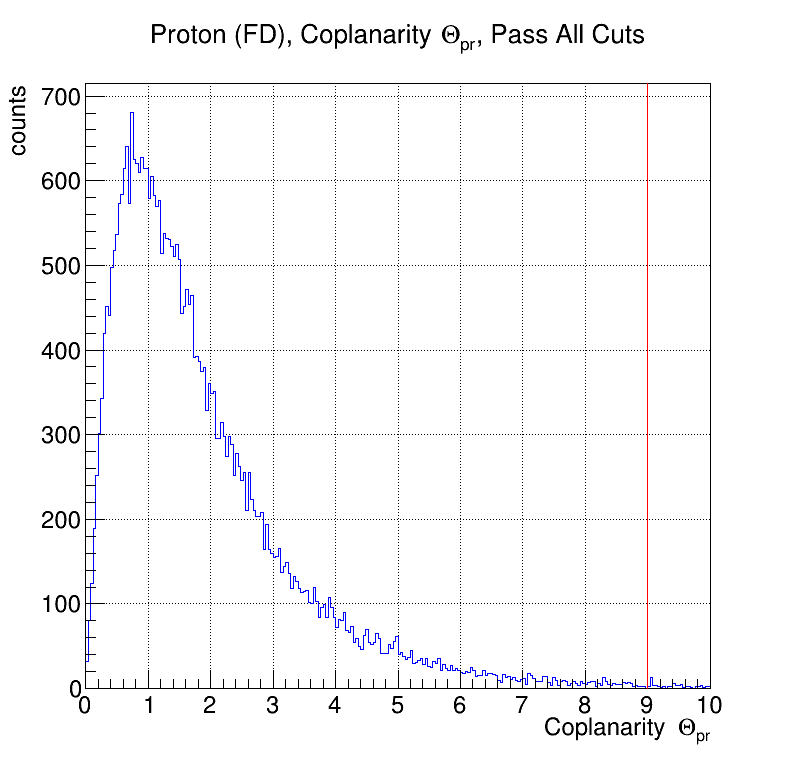
\includegraphics[width=0.565\textwidth]{pdfs/35a.png}
%     \end{figure}\vspace{-0.80cm}
%     \begin{figure}
%         \centering
%         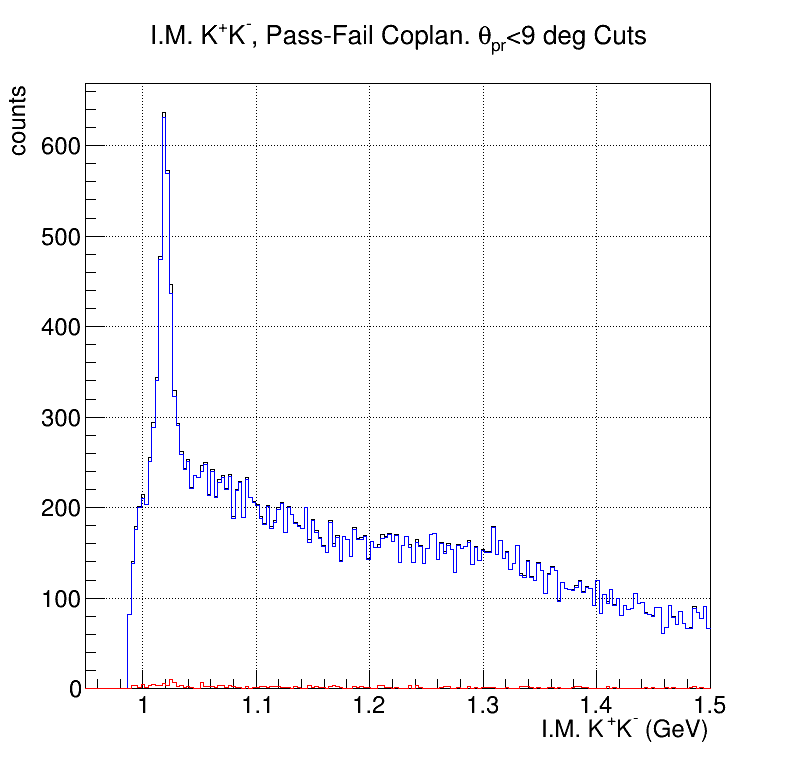
\includegraphics[width=0.565\textwidth]{pdfs/35b.png}
%         \caption{My Reproduction}
%     \end{figure}
%     \end{columns}
% \end{frame}